\documentclass{article}
\usepackage{graphicx} % Required for inserting images
\usepackage{xcolor}
\usepackage{dashbox}
\usepackage{tikz}
\usetikzlibrary{patterns}
\usepackage{xspace}
\usepackage{booktabs,multicol}
\usepackage{mdframed}
\usepackage{hyperref}
\hypersetup{
    colorlinks=true,
    linkcolor=blue,
    filecolor=magenta,
    urlcolor=blue,
    citecolor=blue,
}
\usepackage{amsthm}
\newtheorem{definition}{Definition}
\newtheorem{theorem}{Theorem}
\usepackage{amsmath,amsfonts,amssymb}
\usepackage{wasysym}
\usepackage{cleveref}
\usepackage[lambda]{cryptocode}
\usepackage{hyphenat}
\hyphenation{inter-active}
\hyphenation{block-chain}

% protocol names
\newcommand{\AAL}{A$^2$L\xspace}
\newcommand{\AALplus}{A$^2$L$^+$\xspace}
\newcommand{\AALUC}{A$^2$L$^{\rm UC}$\xspace}
\newcommand{\COCO}{C\ensuremath{\emptyset}C\ensuremath{\emptyset}}

% checkmarks / x's
\usepackage{pifont}
\newcommand{\cmark}{\ding{51}}%
\newcommand{\xmark}{\ding{55}}%

% variables
% \renewcommand{\epsilon}{\varepsilon}

% math
\newcommand{\ZZ}{\ensuremath{\mathbb{Z}}}
\newcommand{\NN}{\ensuremath{\mathbb{N}}}
\newcommand{\GG}{\ensuremath{\mathbb{G}}}
\newcommand{\JJ}{\ensuremath{\mathbb{J}}}
\newcommand{\prob}[1]{\ensuremath{\Pr\left[#1\right]}}
\newcommand{\suchthat}{\ensuremath{\mathrm{~s.t.~}}}
\newcommand{\F}{\ensuremath{\mathcal{F}}}
\newcommand{\X}{\ensuremath{\mathcal{X}}}
\newcommand{\Y}{\ensuremath{\mathcal{Y}}}
\newcommand{\Z}{\ensuremath{\mathcal{Z}}}
\DeclareMathOperator*{\argmax}{arg\,max}
\newcommand{\sizeof}[1]{\lvert #1 \rvert}
\newcommand{\ceil}[1]{\lceil #1 \rceil}

% theorem, etc. environments
\newtheorem{construction}{Construction}
\crefname{construction}{construction}{constructions}
\Crefname{construction}{Construction}{Constructions}

% primitives
\newcommand{\ENC}{\ensuremath{\mathsf{E}}}
\newcommand{\ADP}{\ensuremath{\mathsf{ADP}}}
\newcommand{\DS}{\ensuremath{\mathsf{ADP}}}
\newcommand{\NIZK}{\ensuremath{\mathsf{NIZK}}}
\newcommand{\BCS}{\ensuremath{\mathsf{BCS}}}

%%% cryptography
\newcommand{\negln}[1]{\ensuremath{\mathsf{negl}_{#1}}}
\newcommand{\neglnf}[1]{\ensuremath{\mathsf{negl}_{#1}(\secpar)}}
\newcommand{\negl}{\ensuremath{\mathsf{negl}(\secpar)}}
\newcommand{\adv}{\ensuremath{\mathcal{A}}}
% \newcommand{\secpar}{\ensuremath{\lambda}}
% \newcommand{\secparam}{\ensuremath{1^\secpar}}
\newcommand{\sample}{\ensuremath{\stackrel{\$}{\gets}}}
\newcommand{\randout}{\ensuremath{\stackrel{\$}{\to}}}
\newcommand{\Rel}{\ensuremath{\mathcal{R}}}
\newcommand{\Lang}{\ensuremath{\mathcal{L}}}
% oracles
\newcommand{\oracle}{\ensuremath{\mathcal{O}}}
\newcommand{\oaal}{\ensuremath{\oracle^{\sf A^2L}}}
% common algorithms
\newcommand{\setup}{\ensuremath{\mathsf{Setup}}}
\newcommand{\kgen}{\ensuremath{\mathsf{KGen}}}
\newcommand{\enc}{\ensuremath{\mathsf{Enc}}}
\newcommand{\dec}{\ensuremath{\mathsf{Dec}}}
\newcommand{\ext}{\ensuremath{\mathsf{Ext}}}
\newcommand{\sign}{\ensuremath{\mathsf{Sign}}}
\newcommand{\vrfy}{\ensuremath{\mathsf{Vrfy}}}
\newcommand{\prove}{\ensuremath{\mathsf{P}}}
\newcommand{\recon}{\ensuremath{\mathsf{Reconstruct}}}
% keys
\newcommand{\vk}{\ensuremath{\mathsf{vk}}}
\newcommand{\sk}{\ensuremath{\mathsf{sk}}}
\newcommand{\ek}{\ensuremath{\mathsf{ek}}}
\newcommand{\dk}{\ensuremath{\mathsf{dk}}}
% other elements
\newcommand{\crs}{\ensuremath{\mathsf{crs}}}
\newcommand{\pp}{\ensuremath{\mathsf{pp}}}
\newcommand{\com}{\ensuremath{\mathsf{com}}}
% UC framework
\newcommand{\Sim}{\ensuremath{\mathcal{S}}}
\newcommand{\env}{\ensuremath{\mathcal{E}}}
\newcommand{\real}{\ensuremath{\textsc{real}}}
\newcommand{\ideal}{\ensuremath{\textsc{ideal}}}

%%%%% UC-SE specific stuff %%%%%
\newcommand{\fnizk}{\mathcal{F}_{\mathsf{NIZK}}}
\newcommand{\fupcrs}{\mathcal{F}_{\mathsf{up\text{-}CRS}}}

%%%%% BCS specific stuff %%%%%
\newcommand{\alice}{\ensuremath{\mathit{A}}}
\newcommand{\bob}{\ensuremath{\mathit{B}}}
% adaptor sigs
\newcommand{\presign}{\ensuremath{\mathsf{PreSig}}}
\newcommand{\prevrfy}{\ensuremath{\mathsf{PreVrfy}}}
\newcommand{\adapt}{\ensuremath{\mathsf{Adapt}}}
\newcommand{\presig}{\ensuremath{\tilde{\sigma}}}
% BCS algos
\newcommand{\Promise}{\ensuremath{\mathsf{PPromise}}}
\newcommand{\Pay}{\ensuremath{\mathsf{PSolver}}}
% BCS games
\newcommand{\expUnlink}{\ensuremath\mathsf{ExpBlnd}}
\newcommand{\expUnlock}{\ensuremath\mathsf{ExpUnlock}}
\newcommand{\expSec}{\ensuremath\mathsf{ExpUnforg}}
\newcommand{\Fbcs}{\ensuremath{\mathcal{F}_{\sf BCS}}}

%%%%% Cicada %%%%%
% HTLPs
\newcommand{\htlp}{\ensuremath{\mathsf{HTLP}}\xspace}
\newcommand{\tlp}{\ensuremath{\mathsf{TLP}}\xspace}
\newcommand{\Ttime}{\ensuremath{T}}
% Cicada syntax
\newcommand{\Setup}{\ensuremath{\mathsf{Setup}}}
\newcommand{\Seal}{\ensuremath{\mathsf{Seal}}}
\newcommand{\Aggr}{\ensuremath{\mathsf{Aggr}}}
\newcommand{\Open}{\ensuremath{\mathsf{Open}}}
\newcommand{\Finalize}{\ensuremath{\mathsf{Finalize}}}
\newcommand{\open}{\ensuremath{\mathsf{open}}}

\newcommand{\Score}{\ensuremath{\Sigma}}
\newcommand{\tally}{\ensuremath{t}}
\newcommand{\final}{\ensuremath{f}}
%%pack and unpack functions
\newcommand{\PSetup}{\mathsf{PSetup}}
\newcommand{\pack}{\mathsf{Pack}}
\newcommand{\unpack}{\mathsf{Unpack}}
% sigma protocols
\newcommand*{\poe}{\ensuremath{\mathsf{PoE}}}

%%%%% KSP %%%%%
\newcommand{\hot}{\ensuremath{\mathsf{hot}}}
\newcommand{\cold}{\ensuremath{\mathsf{cold}}}
\newcommand{\skref}{\ensuremath{\mathsf{SKRefresh}}}
\newcommand{\shref}{\ensuremath{\mathsf{ShareRefresh}}}
\newcommand{\cSign}{\mathsf{CSign}\xspace}
\newcommand{\hSign}{\mathsf{HSign}\xspace}
\newcommand{\hx}{\tilde{x}}
\newcommand{\aux}{\mathsf{aux}}
\newcommand{\cProof}{\mathsf{CProof}\xspace}
\newcommand{\hProof}{\mathsf{HProof}\xspace}
\newcommand{\timeT}{\ensuremath{T}}
\newcommand{\copied}[1]{\textcolor{red}{[copied] #1}}
\newcommand{\noemi}[1]{\textcolor{magenta}{Noemi: #1}}
\newcommand{\todo}[1]{\textcolor{red}{todo: #1}}

\title{Cryptography for Private and Secure Blockchain Applications}
% \title{Cryptography for Blockchain Applications}
% \title{Privacy-Enhancing Technologies for Blockchains}
% \title{Improving Privacy and Security of Blockchain with Cryptography}
% \title{Private and Responsible Decentralized Payments} % from MPI contract
\author{Noemi Glaeser}
\date{}

\begin{document}

\maketitle
\begin{abstract}
In 2008, Satoshi Nakamoto introduced Bitcoin, the first digital currency without a trusted authority whose security is maintained by a decentralized blockchain. Since then, a plethora of decentralized applications have been proposed utilizing blockchains as a public bulletin board. In recent years, it has become clear that this basic functionality is not enough to prevent widespread attacks on both the privacy and security of blockchain users, as evidenced by the blockchain analytics industry and the billions of dollars stolen via cryptocurrency exploits to date. 

This work explores the role cryptography has to play in the blockchain ecosystem to both enhance user privacy and secure user funds. I discuss how to generically add universally composable security to any non-interactive zero-knowledge proof (NIZK), a crucial building block in many blockchain systems, in a way that is compatible with an updatable common reference string. This strengthens security for any system relying on NIZKs, including many blockchains and blockchain applications, while maintaining minimal trust assumptions. Next, I discuss how to improve the security of a class of coin mixing protocols by giving a formal security treatment of this class and patching the security of an existing, insecure protocol. Finally, I show how to construct efficient, non-interactive, and private on-chain protocols for a large class of elections and auctions. I conclude by describing two proposed works: a new threshold wallet construction and a systematic comparison of on-chain key management approaches.

% Blockchains are inherently public, [but sometimes we want privacy. We need to use crypto to do this. And so on and so forth\dots] \noemi{actually probably need to expand to also include ``security'', since the threshold sigs project isn't really about privacy}
% A key challenge in [my area of research] is [problem I halfway figured out how to solve]. (And so on and so forth\dots)
\end{abstract}

\tableofcontents
\newpage

In most blockchains with programming capabilities, e.g., Ethereum~\cite{ethereum_yellowpaper}, developers are incentivized to minimize the storage and computation complexity of on-chain programs. Applications with high compute or storage incur significant fees, commonly referred to as \emph{gas}, to compensate validators in the network. Often, these costs are passed on to users of an application. 

High gas costs have motivated many applications to utilize \emph{verifiable computation (VC)}~\cite{C:GenGenPar10}, off-loading expensive operations to powerful but untrusted off-chain entities who perform arbitrary computation and provide a short proof\footnote{More precisely, a succinct non-interactive argument of knowledge, or SNARK.} that the claimed result is correct.
This computation can even depend on secret inputs not known to the verifier by relying on zero-knowledge proofs (i.e., zkSNARKs).
 %In some cases (though not all), this proof is also zero-knowledge, hiding some inputs to the computation. This is commonly referred to as a \emph{zk-rollup} (even if it is not zero-knowledge).

 \begin{figure}[tbh]
    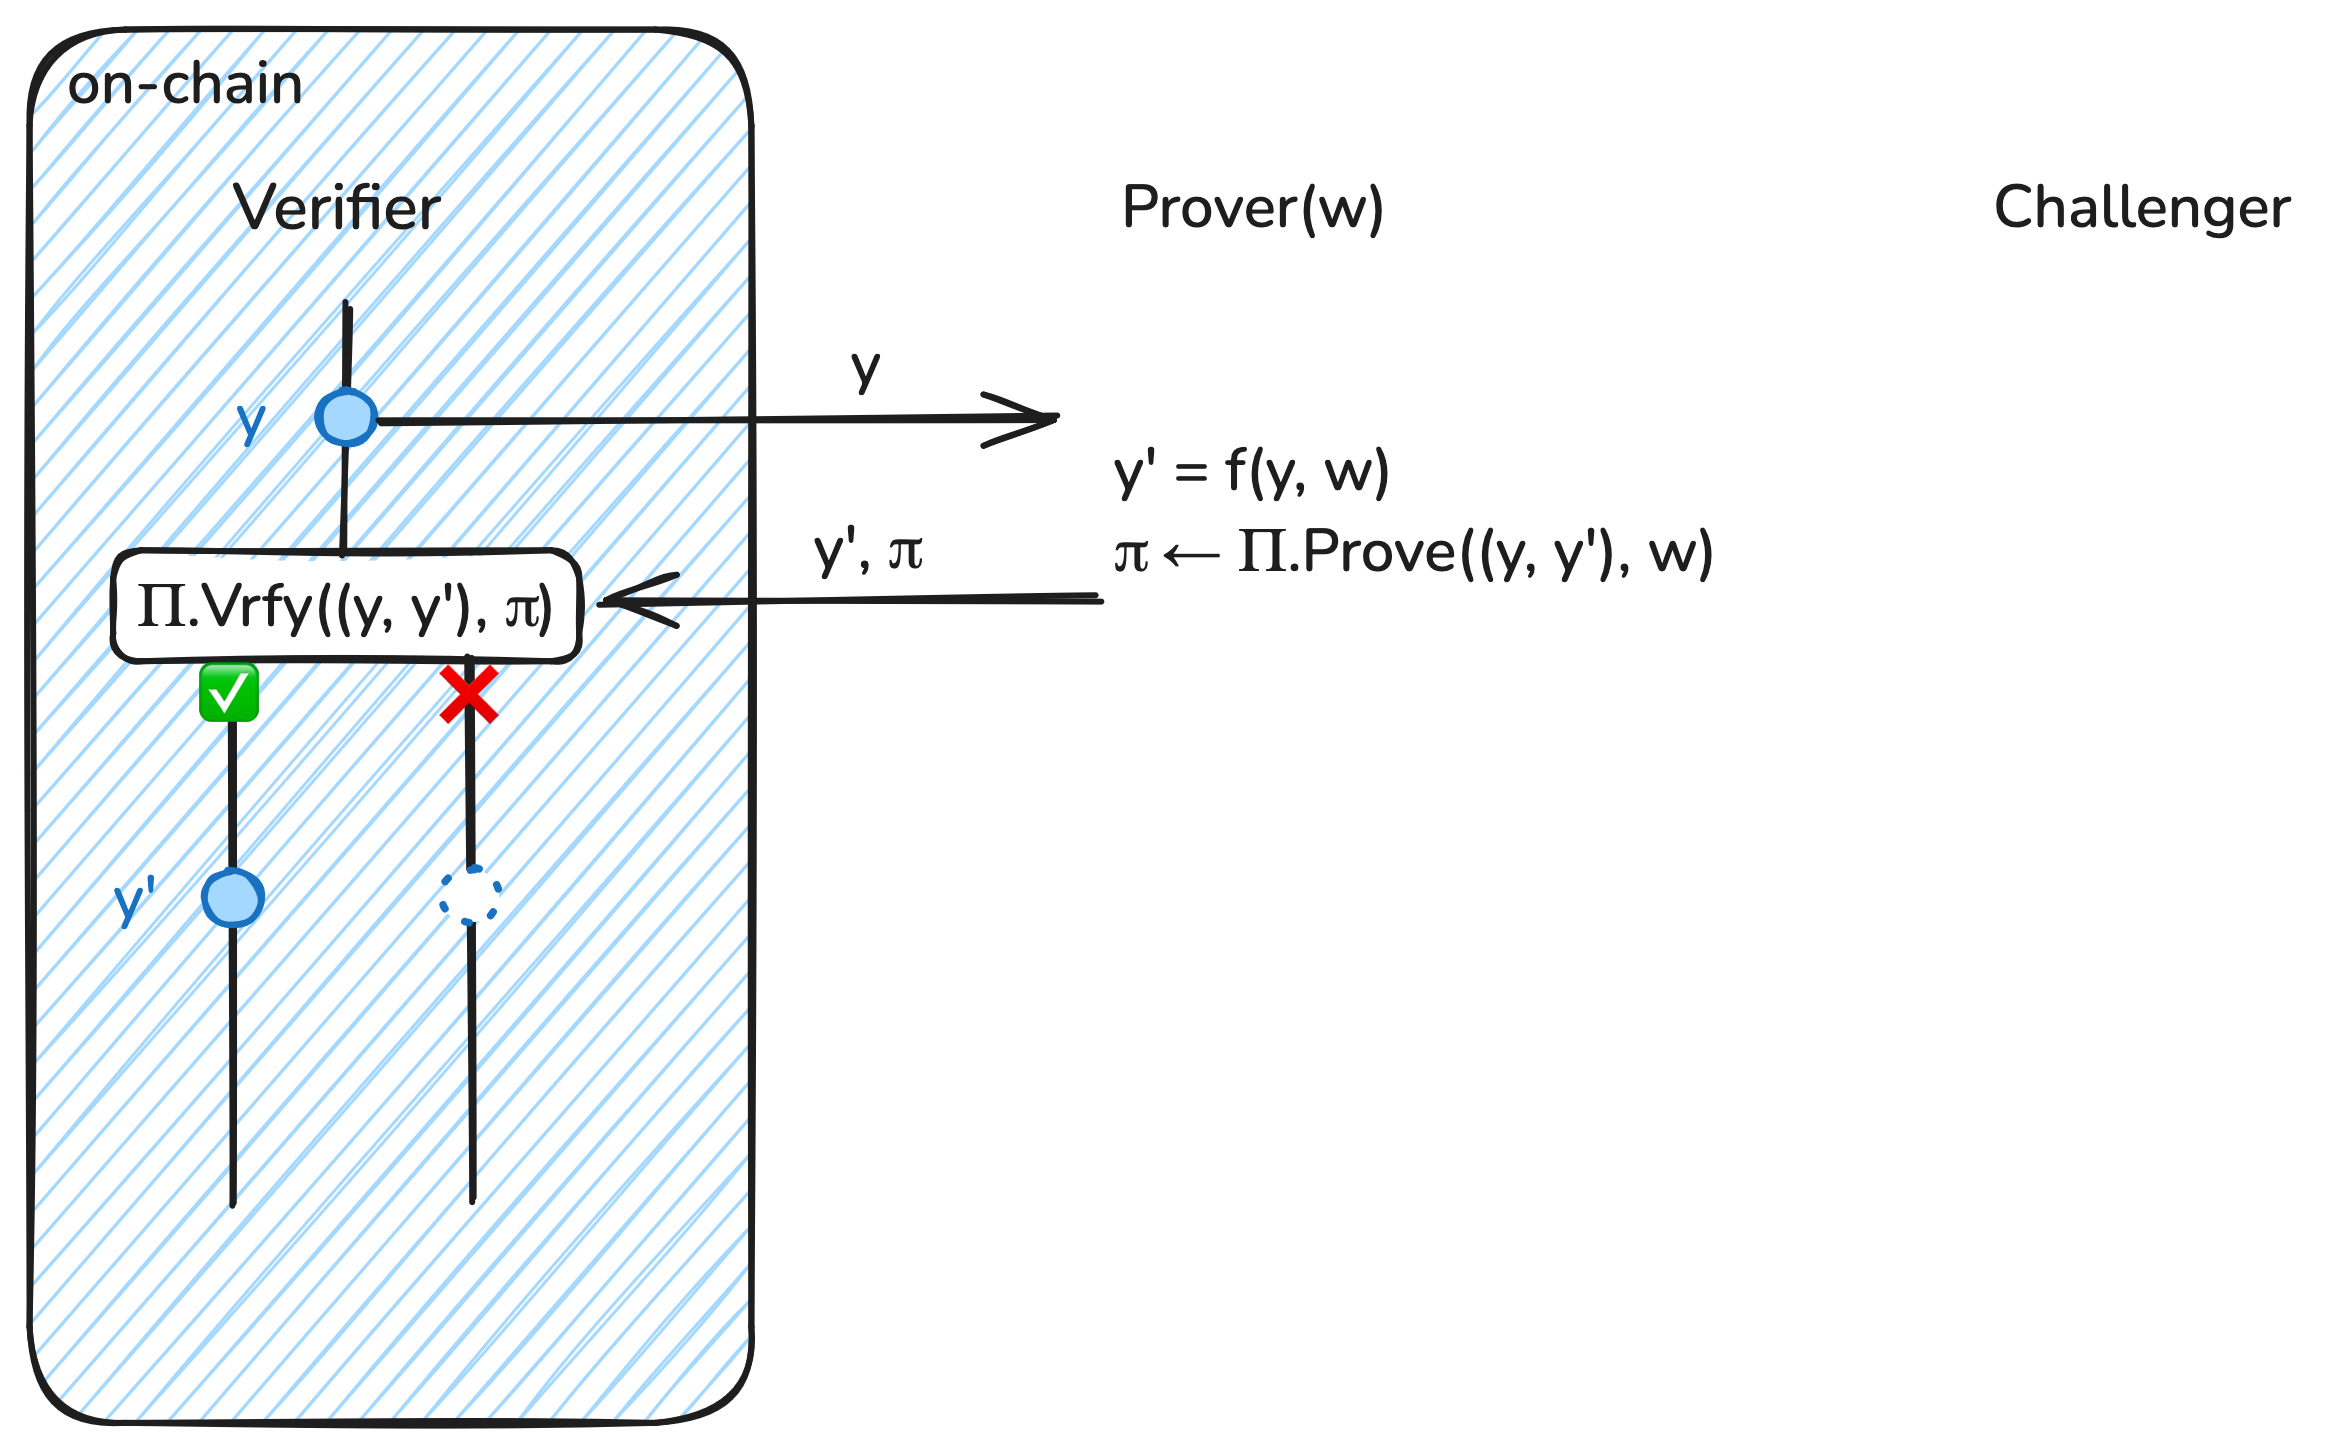
\includegraphics[width=\textwidth]{naysayer/figs/vc.png}
    \caption{\textbf{Using VC to move computation off-chain.} The off-chain ``prover'' applies the function $f$ to input $y$ and potentially an auxiliary off-chain input $w$ to get the result $y' = f(y, w)$. (In the case of a zk-rollup, $f$ is the state transition function, $y$ is the previous on-chain state, $w$ is a batch of transactions, and $y'$ is the new state after applying the transactions in $w$ to $y$.) It posts $y'$ and a proof $\pi$ of its correctness, which is verified on-chain before the output $y'$ is accepted. This paradigm does not require any challengers.\todo{update $\sf Vrfy$ to $\vrfy$ in fig}}
    \label{fig:vc}
 \end{figure}

VC leads to a paradigm in which smart contracts, while capable of arbitrary computation, primarily act as verifiers and outsource all significant computation off-chain (see \Cref{fig:vc}). A motivating application is so-called ``zk''-\emph{rollups}\footnotemark~\cite{starknet,zksync,aztec,dydx,scroll}, which combine transactions from many users into a single smart contract which verifies a proof that all have been executed correctly.
\footnotetext{The ``zk'' part of the name is often a misnomer, since these services do not necessarily offer the zero-knowledge property, and in fact most do not.} 
However, verifying these proofs can still be costly. For example, the StarkEx rollup 
%contract verifying the state transitions of the off-chain StarkEx marketplace 
has spent hundreds of thousands of dollars to date to verify FRI polynomial commitment opening proofs.\footnote{\url{https://etherscan.io/address/0x3e6118da317f7a433031f03bb71ab870d87dd2dd}}
% Even verifying simple statements can exceed the block gas limit of Ethereum~\cite{EPRINT:NRBB22}\todo{not sure about this example. Maybe a dollar figure on STARKs would more convincing?}\istvan{I had in mind the CRS for EIP-4844 that would have been exceeded the block gas limit with this solution.}.

We observe that this proof verification is often wasteful. In most applications, provers have strong incentives to post only correct proofs, suffering direct financial penalties (in the form of a lost security deposit) or indirect costs to their reputation and business for posting incorrect proofs. As a result, a significant fraction of a typical layer-1 blockchain's storage and computation is expended verifying proofs, which are almost always correct.\footnote{At the time of this writing, we are unaware of any major rollup service which has posted an incorrect proof in production.}

 \begin{figure}[tb]
    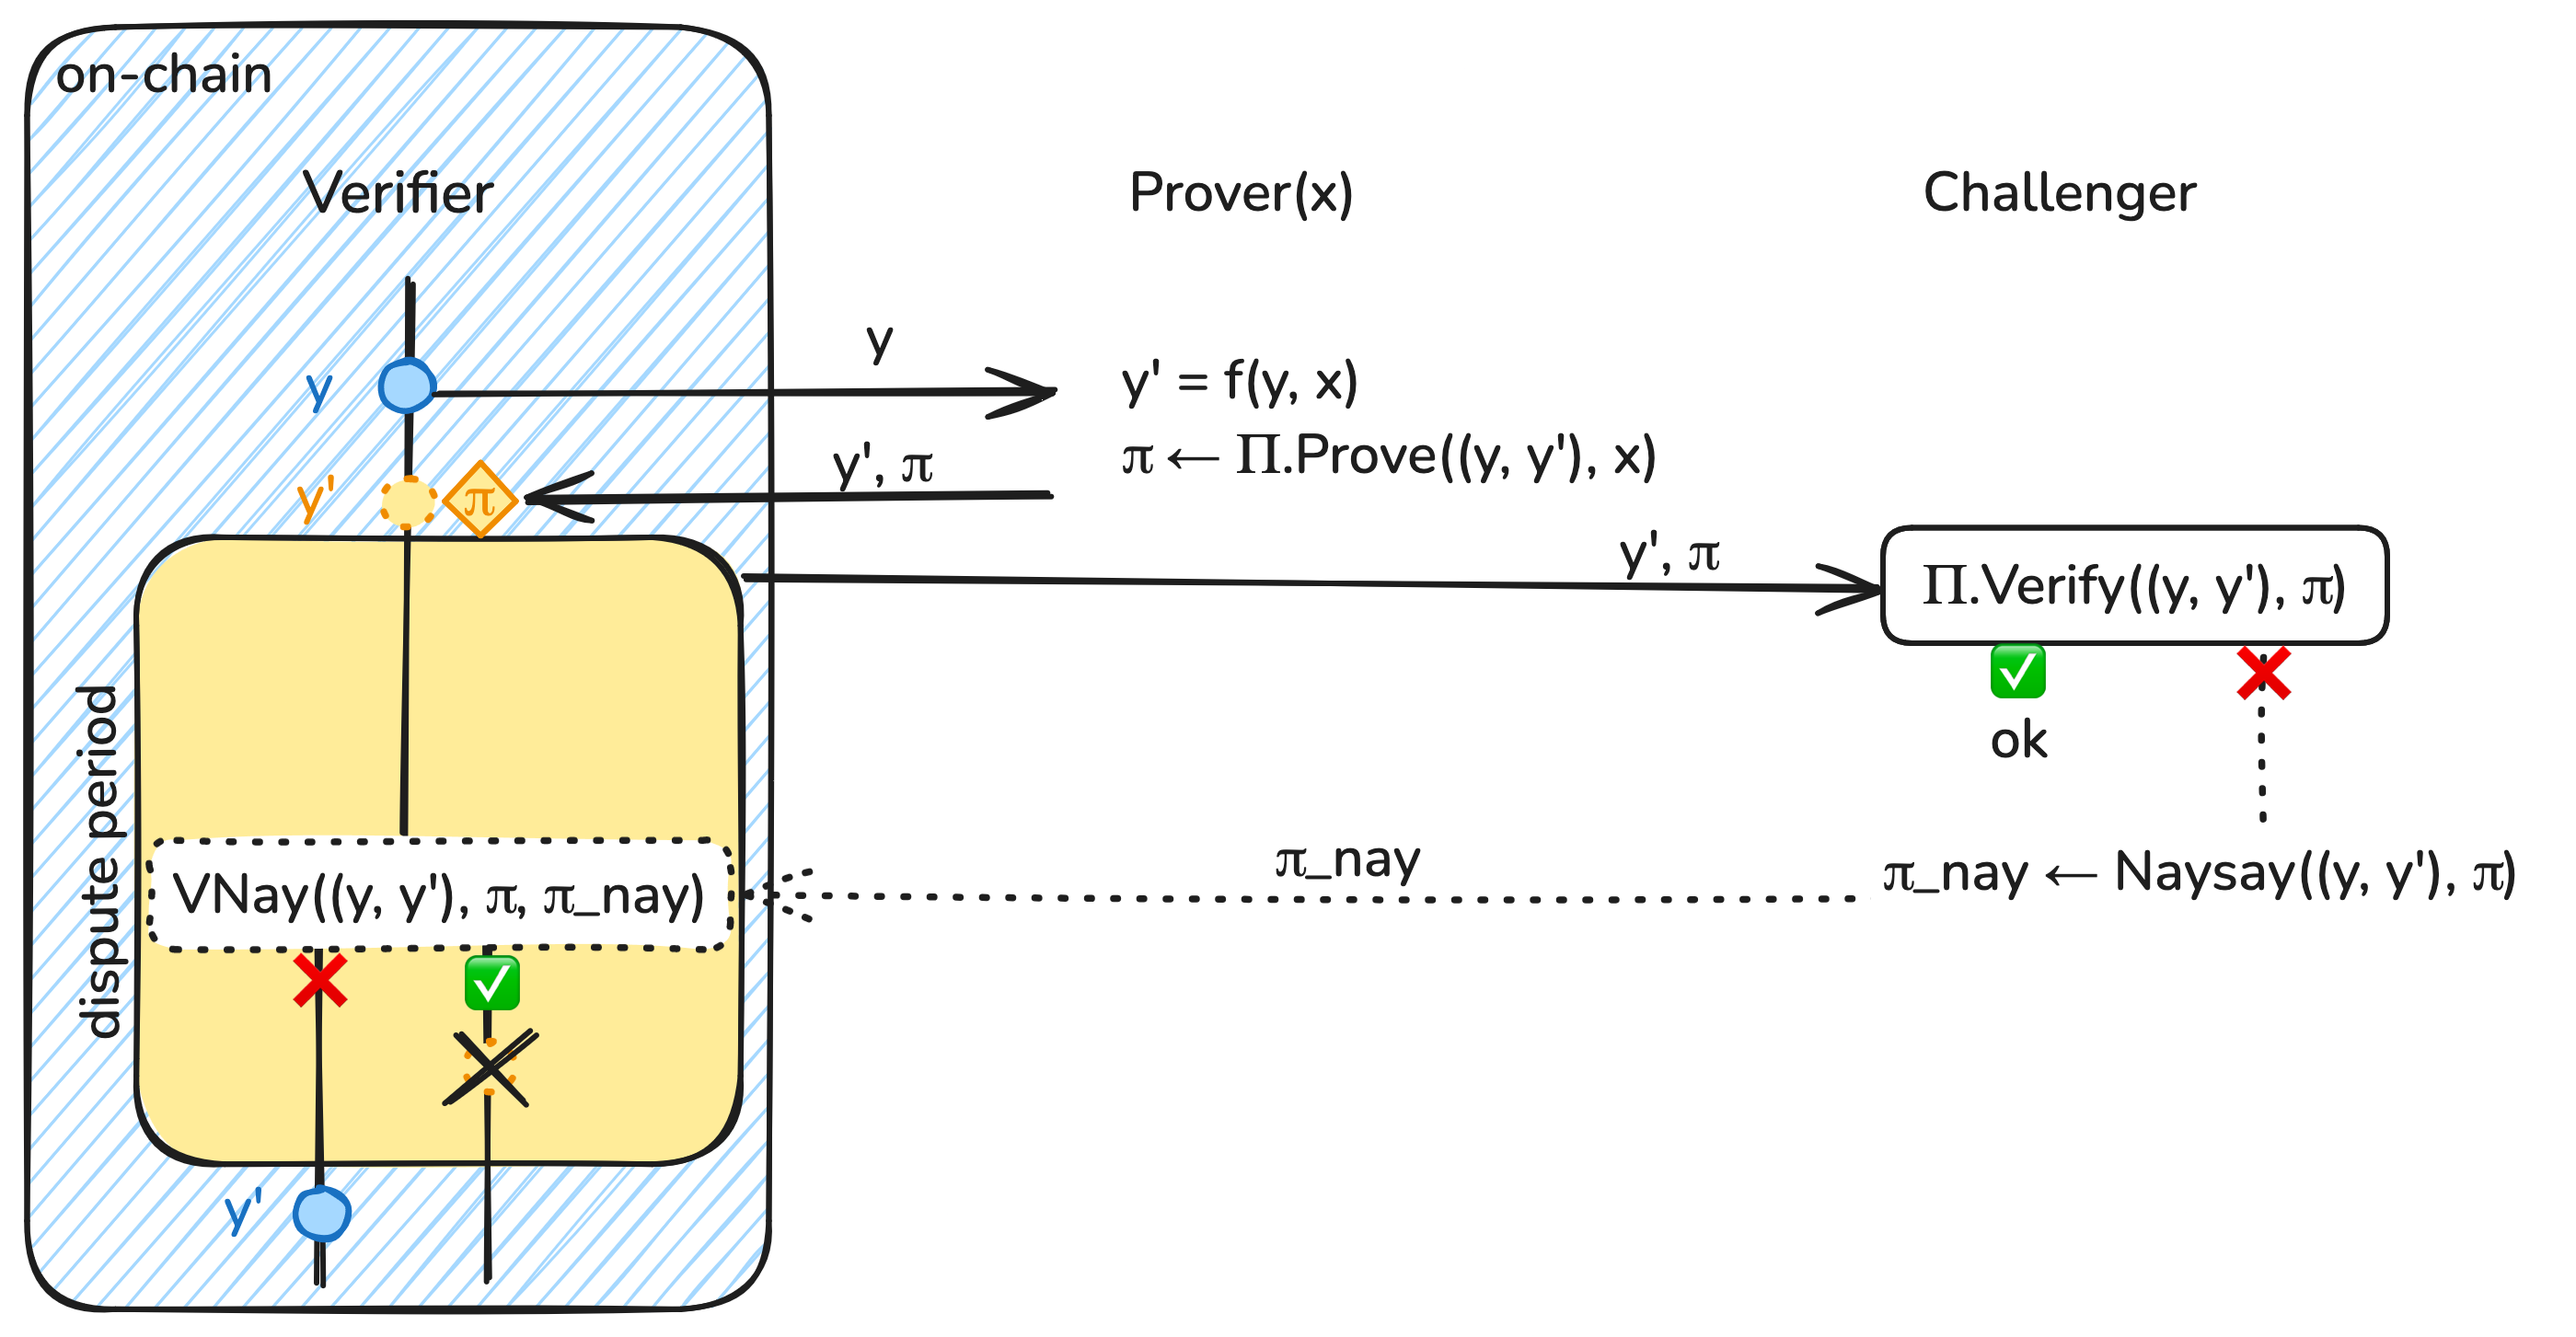
\includegraphics[width=\textwidth]{naysayer/figs/naysayer.png}
    \caption{\textbf{The naysayer proof approach.} As in VC, the off-chain prover computes $y' = f(y, w)$ and $\pi$, which it posts on-chain. This time, the proof is \emph{not} verified on-chain, but is provisionally accepted while waiting for the challenge period to pass. Any party can verify $\pi$ off-chain and, if it fails, issue a challenge by creating a naysayer proof $\pi_\nay$. The on-chain verifier checks any submitted naysayer proofs, and if they pass, it rejects the claimed result $y'$. If the challenge period elapses without any successful naysaying, $y'$ is accepted.}
    \label{fig:naysayer}
 \end{figure}

This state of affairs motivates us to propose a new paradigm called \emph{naysayer proofs} (\Cref{fig:naysayer}). In this paradigm, the verifier (e.g., a rollup smart contract) optimistically accepts a submitted proof without verifying its correctness. Instead, any observer can check the proof off-chain and, if needed, prove its \emph{incorrectness} to the verifier by submitting a \emph{naysayer proof}. The verifier then checks the naysayer proof and, if it is correct, rejects the original proof.
Otherwise, if no party successfully naysays the original proof before the end of the challenge period, the original proof is accepted.
To deter denial of service, naysayers may be required to post collateral, which is forfeited if their naysayer proof is incorrect.

This paradigm potentially saves the verifier work in two ways. 
First, in the optimistic case, where the proof is not challenged, the verifier does no work at all (just like the related fraud proof paradigm; see \Cref{sec:naysayer_related}). We expect this to almost always be the case in practice. Second, even in the pessimistic case, we will see below that checking the naysayer proof can be much more efficient than checking the original proof.
In other words, the naysayer acts as a helper to the verifier by reducing the cost of the verification procedure in fraudulent cases. At worst, checking the naysayer proof is equivalent to verifying the original proof (this is the trivial naysayer construction).

Naysayer proofs enable other interesting trade-offs. 
% for instance, %for a proof system with transparent setup and large proofs, the \naysayer proof could be instantiated generically using a short proof system with trusted setup (e.g., \cite{groth16}), or using a lower security level. 
For instance, naysayer proofs can be instantiated with a lower security level than the original proof system.
This is because a violation of the naysayer proof system's soundness undermines only the \emph{completeness} of the original proof system. %, but not its soundness. 
For an application like a rollup service, this would result in a loss of liveness; importantly, the rollup users' funds would remain secure. 
Liveness could be restored by falling back to full proof verification on-chain.

%Move this to later? Conclusion?
%The naysayer paradigm introduces a new set of criteria for evaluating the efficiency of proof systems. Previously, developers were solely focusing on the proof size and verification cost of a proof system; this paradigm allows one to instead optimize for a proof system's proof size \emph{and its accompanying naysayer proof size and verification cost}. We further detail the implications of these new selection criteria in~\Cref{sec:evaluation}.

We will formally define naysayer proofs in~\Cref{sec:naysayer_def} and show that every succinct proof system has a logarithmic-size and constant-time naysayer proof. Before that, we discuss related work in \Cref{sec:naysayer_related} and define our system model in more detail in \Cref{sec:naysayer_model}.
In~\Cref{sec:naysayer_apps}, we construct naysayer proofs for four concrete proof systems and evaluate their succinctness. % in comparison with verifying the original proof. 
We discuss storage considerations in \Cref{sec:naysayer_storage} and conclude with some open directions in~\Cref{sec:naysayer_extensions}.

\section{Privacy-Enhancing Building Blocks}\label{sec:building-blocks}

Although cryptocurrencies are often treated as fully anonymous digital currencies, numerous works have shown how to link transactions or even fully deanonymize users on many popular blockchains \cite{CCS:BirKhoPus14,EuroSP:BirTik19,FC:KosKosMcD14,PoPETS:MSHLHSHHMNC18,USENIX:KYMM18}. Numerous mitigations have been suggested, including adding privacy as an overlay on top of existing blockchains (e.g., via cryptocurrency mixers, described in \Cref{sec:mixers}), or by building new privacy-first cryptocurrencies like Zcash~\cite{zcash} and Monero~\cite{monero}. Many of these overlays and new blockchains rely on zero-knowledge proofs.

\subsection{Zero-Knowledge Proofs and their trust assumptions}

Non-interactive zero-knowledge proofs (NIZKs) are ubiquitous building blocks for achieving both privacy and scalability. Zcash~\cite{zcash} relies heavily on a type of NIZK called a zk-SNARK (zero-knowledge succinct non-interactive argument of knowledge) to prove that a party has sufficient funds to make a payment without revealing anything more about those funds~\cite{SP:BCGGMT14}. On Ethereum, so-called (zk-)rollups enhance scalability by leveraging the succinctness of (zk-)SNARKs, though they may or may not offer the zero-knowledge property.

To achieve such a high level of succinctness, SNARKs rely on a trusted setup to generate a \emph{common reference string (CRS)}. In keeping with the primary innovation of the blockchain, which is the elimination of a trusted third party, practitioners use various approaches to minimize trust in the CRS generation. Zcash uses a multi-party computation ceremony~\cite{zcash-ceremony} with many independent participants to distribute the trust among several parties. Another trust-minimizing approach consists of using SNARKs with universal and updatable CRS~\cite{C:GKMMM18,CCS:MBKM19,EC:CHMMVW20,EPRINT:GabWilCio19}. A universal CRS can be reused across applications, avoiding a new complicated setup ceremony for every use. Updatable CRSs allow any participant in a system to contribute randomness to the CRS at any point, including once the CRS is in production use, to enable a ``one-out-of-many'' trust scenario in which the user must only trust themselves to contribute (and then delete) good randomness to the CRS in order for the whole system to be secure.

An orthogonal concern is maintaining the security of SNARKs when they are composed with other protocols in the complex blockchain ecosystem. Formally, this is modeled by universally composable security via the universal composability (UC) framework~\cite{FOCS:Canetti01}. Unfortunately, most SNARKs in deployment today are not provably UC-secure. Although compilers to transform any SNARK or NIZK into a UC variant exist~\cite{EPRINT:KZMQCP15,EC:GKOPTT23}, these are not compatible with the aforementioned trust-minimizing properties like updatability. A generic compiler which adds UC-security while maintaining updatability would help ensure confidence in both the trusted setup and the operational security of deployed NIZKs.

\renewcommand{\cmark}{\CIRCLE}
\renewcommand{\xmark}{\Circle}
\begin{table}[tbh]
    \centering
    \begin{tabular}{l@{\hspace{1em}} cc cc c}
        \toprule
        & \multicolumn{2}{c}{UC} & \multicolumn{2}{c}{succinctness-preserving}    & \\ \cmidrule(r{3pt}){2-3} \cmidrule(l{3pt}){4-5}
        & SE     & BBE    & in $\lvert C \rvert$ & in $\lvert w \rvert$ & upd. CRS \\
        \midrule
        \COCO~\cite{EPRINT:KZMQCP15}    & \cmark & \cmark & \cmark           & \xmark           & \xmark\\
        DS~\cite{DCC:DerSla19}          & \cmark & \xmark & \cmark           & \cmark           & \xmark\\
        \textsc{Lamassu}~\cite{CCS:AbdRamSla20} & \cmark & \xmark & \cmark           & \cmark           & \cmark\\
        \midrule
        This work \cite{CSF:AGRS24}     & \cmark & \cmark & \cmark           & \xmark           & \cmark\\
        Concurr. work~\cite{EC:GKOPTT23} & \cmark & \cmark & \cmark           & \cmark           & \xmark\\
        \bottomrule
    \end{tabular}
    \caption{Comparison with concurrent and previous work. SE = simulation extractability, BBE = black-box extractability.}\label{tab:comparison}
\end{table}

\subsubsection{Contribution: Circuit-succinct universally composable NIZKs with updatable CRS}

\textit{(Parts of this section are taken/adapted from \cite{CSF:AGRS24}.)}

\usetikzlibrary{fit}
\begin{figure}[tbh]
    \begin{center}
        \begin{tikzpicture}
            \node[draw] (crs_enc) {$\crs_\mathit{enc}$};
            \node[draw] (crs_snark) [right=3em of crs_enc] {$\crs_\mathit{SNARK}$};
            \node[draw] (crs_sig) [right=3em of crs_snark] {$\crs_\mathit{sig}$};
            %
            \node[draw,double] (ucrs_enc) [above=2em of crs_enc] {${\sf u}\crs_\mathit{enc}$};
            \node[draw,double] (ucrs_snark) [above=2em of crs_snark] {${\sf u}\crs_\mathit{SNARK}$};
            \node[draw,double] (ucrs_sig) [above=2em of crs_sig] {${\sf u}\crs_\mathit{sig}$};
            %
            \node[draw] (r_enc) [below=2em of crs_enc] {$\land \mathcal{R}_\mathit{enc}$};
            % pattern=north east lines,fill opacity=0.5
            \node[draw,fill=gray!20] (r_snark) [below=2em of crs_snark] {$\mathcal{R}_\mathcal{L}$};
            \node[draw] (r_sig) [below=2em of crs_sig] {$\lor \mathcal{R}_\mathit{sig}$};
            %
            \node[] (center) [right=1em of r_snark] {};
            \node[] (dspadding) [below=1em of center] {};
            \node[draw,fill=blue,opacity=0.2,inner sep=7pt,fit=(crs_snark) (crs_sig) (r_snark) (r_sig) (dspadding)] (ds) {};
            \node[above] at (ds.south) {DS: non-BB SE};
            %
            \node[] (lamassupadding) [below=2.5em of center] {};
            \node[draw,fill=green,opacity=0.2,inner xsep=15pt,inner ysep=10pt,fit=(ucrs_snark) (ucrs_sig) (r_snark) (r_sig) (lamassupadding)] (lamassu) {};
            \node[above] at (lamassu.south) {\textsc{Lamassu}: upd. non-BB SE};
            %
            % \node[] (topmargin) [above=.5em of crs_snark] {};
            \node[] (cocopadding) [below=3.5em of r_snark] {};
            \node[draw,fill=yellow,opacity=0.2,inner xsep=25pt,inner ysep=13pt,fit=(crs_enc) (crs_sig) (r_enc) (r_sig) (cocopadding)] (coco) {};
            \node[above] at (coco.south) {\COCO: BB SE (UC)};
            %
            \node[] (bblamassupadding) [below=5em of r_snark] {};
            \node[draw,inner xsep=35pt,inner ysep=15pt,fit=(ucrs_enc) (ucrs_sig) (r_enc) (r_sig) (bblamassupadding)] (bblamassu) {};
            \node[above] at (bblamassu.south) {This work: upd. BB SE (UC)};
            %
            \draw[->] (crs_enc)--(ucrs_enc);
            \draw[->] (crs_snark)--(ucrs_snark);
            \draw[->] (crs_sig)--(ucrs_sig);
        \end{tikzpicture}
    % trim=left bottom right top
    % 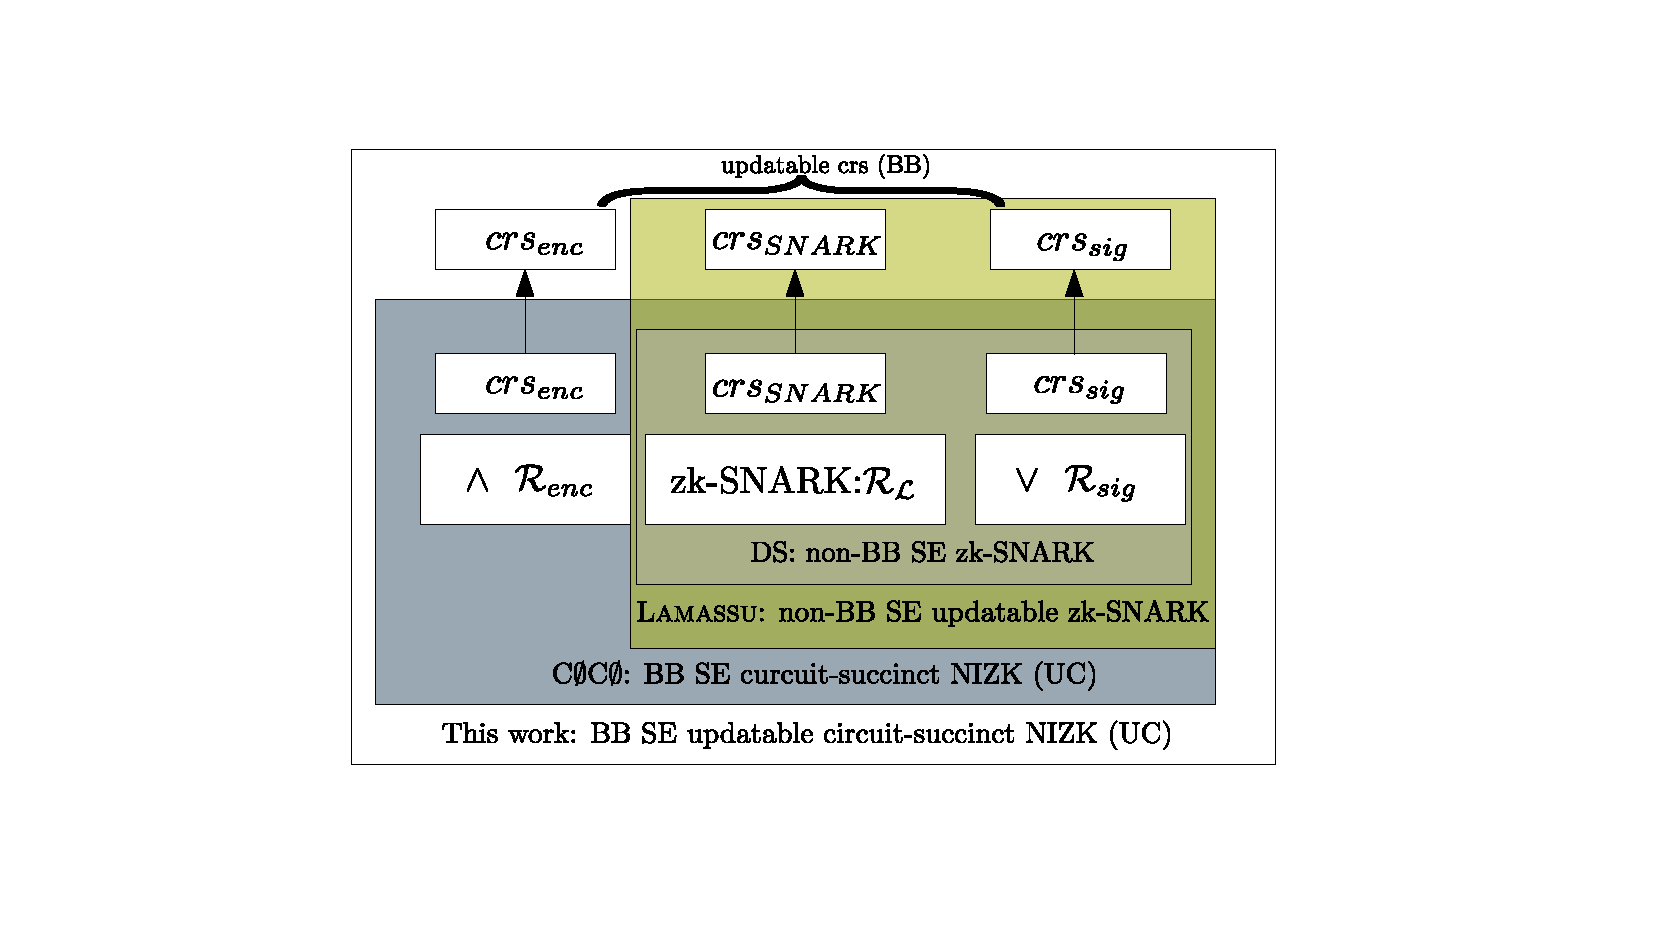
\includegraphics[trim=5.5cm 2.5cm 5cm 2cm, clip, scale =0.5]{overview_new}
    \end{center}
    \caption{Overview of our approach including previous work from Table~\ref{tab:comparison}. ${\sf u}\crs$ denotes an updatable CRS.}
    \label{fig:ucse-overview}
\end{figure}

In \cite{CSF:AGRS24} we show how to build such a compiler by giving the first \emph{fully black-box approach to generically build} circuit-succinct UC-secure NIZKs with updatable CRS from any zk-SNARK, circumventing the aforementioned problems. \textsc{BB-Lamassu} is a framework for black-box (BB) simulation-extractable (SE) (i.e., universally-composable) circuit-succinct NIZKs with updatable CRS. It can be seen as a hybrid of \COCO~\cite{EPRINT:KZMQCP15} and \textsc{Lamassu}~\cite{CCS:AbdRamSla20}, combining the BB extractability of the former with the updatable CRS compatilbility of the latter (see \Cref{tab:comparison}). 
% We follow an approach similar to \COCO\ (grey box) to achieve BB extractability, which as mentioned above requires relaxing the succinctness of SNARKs to that of circuit-succinct NIZKs~\cite{EC:KNYY20} since we need to encrypt the witness in the proof.

\COCO\ (yellow box in \Cref{fig:ucse-overview}) combines two tricks from the literature to achieve BBE and SE. First, to avoid non-black-box extractors that rely on rewinding or knowledge assumptions, they extend the CRS by a public key and include an encryption of the witness in the proof. This also requires extending the original statement to show that the correct witness was encrypted ($\mathcal{R}_{enc}$)~\cite{FOCS:DeSPer92}. Now the extractor can extract the witness by simply decrypting the ciphertext in the CRS. Second, they use the classical OR trick (i.e., an alternate clause $\mathcal{R}_{sig}$, to be used only by the simulator, which checks for a valid signature) to enable unbounded simulation of proofs~\cite{C:DDOPS01}, i.e., SE with a straight-line extractor. Together, these additions augment the underlying scheme with SE and UC-security, but the new ciphertext in the CRS ($\crs_{enc}$) adds a linear overhead of $\sizeof{w}$, so it does not fully preserve succinctness and can only give UC SE \emph{NIZKs}.

\textsc{Lamassu} (green box) revisits the \COCO\ framework, tailoring it to updatable NIZKs and removing the $\sizeof{w}$ overhead. This is achieved by using the non-black-box extractor of the underlying scheme instead of an encryption of the witness, thus preserving succinctness (modulo some small constant overhead). To make unbounded proof simulation compatible with an updatable CRS, \textsc{Lamassu} adapts the simulation technique of \cite{DCC:DerSla19} (blue box), which used the OR trick to combine the underlying SNARK's non-BB extractor with key-homomorphic signatures. To support an updatable CRS, \textsc{Lamassu} swaps the signature for an updatable signature (US). The result is a generic framework for CRS-updatable SE succinct NIZKs, but it sacrifices UC-security due to the non-black-box extractor.

\paragraph{BB-Lamassu.} Our new framework BB-\textsc{Lamassu} (outside box) uses \textsc{Lamassu} as a starting point and adds back in an encryption of the witness ($\mathcal{R}_{enc}$) for BB-extractability. To be compatible with updatability, we instantiate this with a novel public-key encryption (PKE) primitive which we call \emph{extractable key-updatable PKE (EKU-PKE)}, for which we show an efficient construction. 
We still have to overcome the hurdle of providing BB extraction for the US and the public key of the EKU-PKE in the CRS ($crs_{enc}$). In brief, this is done by using an efficient (but not necessarily succinct) BBE NIZK \emph{without a CRS} to prove updates of the CRS elements, i.e., updates of $crs_{SNARK}$, the US public key $crs_{sig}$, and the EKU-PKE public key $crs_{enc}$. 
% \copied{We choose to base these proofs on $\Sigma$-protocols converted to NIZK proofs using either the Fiat-Shamir (FS)~\cite{C:FiaSha86}, Fischlin~\cite{C:Fischlin05} or Unruh~\cite{EC:Unruh15} approach. While this requires that the updates of all components are $\Sigma$-protocol friendly, this holds true for the relations in all known constructions. Interestingly, a byproduct of this approach is that the update proofs for the underlying SNARK CRS become much more efficient to verify (and typically also much smaller). This improvement also carries over to the original \textsc{Lamassu} framework~\cite{CCS:AbdRamSla20} and can be used to improve their CRS update proofs as well.}

\paragraph{UC security proof.}
Since BB-\textsc{Lamassu} is BB SE, it is also UC-secure and should therefore realize the NIZK ideal functionality $\fnizk$ of \cite{AC:Groth06}. However, so far this ignores the updatable CRS aspect. 
To formally confirm this intuition, we introduce a new ideal functionality $\fupcrs$ for the updatable CRS generation and then prove that BB-\textsc{Lamassu} realizes the functionality $\fnizk$ in the $\fupcrs$-hybrid model.
Our analysis is carried out in the local ROM, which can be realized in practice by domain separation in the hash function. We note that the use of an RO arises from a building block (the proof of CRS update) and not from the construction of our compiler. %While we currently consider only the local ROM, we expect that an analysis in the global ROM is possible when relying on Fischlin for the update proofs via the techniques in \cite{TCC:LysRos22}.

\begin{figure}[tb]
    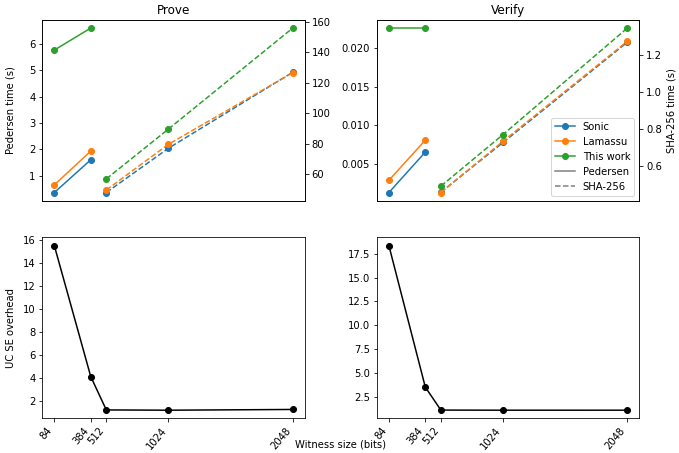
\includegraphics[width=\linewidth]{ucse-benchmarks.png}
    \caption{Runtimes of the Prove and Verify algorithms for Pedersen and SHA-256 preimages using our BB SE succinct NIZK compared to the non-BB SE zk-SNARK obtained via \textsc{Lamassu}~\cite{CCS:AbdRamSla20} and the base non-SE zk-SNARK Sonic~\cite{CCS:MBKM19}. In the lower part we plot the overhead of our transformation to add BB SE, which decreases as the witness size increases.}
    % We do not plot Helped Verify times because they are very small (on the order of hundreds of $\mu$s) and any pattern is overshadowed by noise.
    \label{fig:ucse-eval}
\end{figure}

\paragraph{Performance evaluation.} To demonstrate the applicability of BB-\textsc{Lamassu}, we provide a detailed analysis of the induced overheads. 
For concrete instantiations, we estimate overheads of 32 bytes for the CRS, 170 bytes for the CRS update, and 256 bytes plus the size of the witness for the proof. This is a reduction in both storage and runtime overheads compared to \textsc{Lamassu}~\cite{CCS:AbdRamSla20}.
For witness sizes observed in practical applications such as Zcash, BB-\textsc{Lamassu} adds well below 10,000 additional constraints.

As a concrete example, we apply BB-\textsc{Lamassu} to Sonic~\cite{CCS:MBKM19}, a zk-SNARK with updatable CRS.\footnote{\url{https://github.com/nglaeser/sonic-ucse/}} 
We then experimentally evaluate the overhead introduced by BB-\textsc{Lamassu}. For a SHA-256 preimage, which is interesting for Merkle-tree membership proofs, the prover and verifier overhead, respectively, is $\approx 1.2\times$ and $1.07\times$. Our evaluation shows that as the circuits become larger and more complex, proving and verifying the original circuit dominates the overall performance costs and the overhead added by BB-\textsc{Lamassu} converges to the size of the witness (see \Cref{fig:ucse-eval}).

\section{Privacy-Enhancing Applications}\label{sec:applications}

Because the blockchain itself does not guarantee the privacy of users, privacy is often added at the application layer. For example, many applications serve as a privacy overlay to the underlying payment layer. Other applications, such as private voting, enable a wholly new functionality while also adding privacy.

% \subsection{Anonymous Atomic Locks for coin mixing and cross-chain payments}
\subsection{Cryptocurrency Mixers}\label{sec:mixers}

\textit{(Parts of this section are taken/adapted from \cite{CCS:GMMMTT22}.)}

% \noemi{How to position this? Our focus will be on \emph{off-chain} mixers, whose focus is on enabling \emph{scalability} and \emph{interoperability} rather than privacy...}
% \todo{Talk about how these also solve scalability and interoperability?}

Cryptocurrency mixers~\cite{ESORICS:RufMorKat14,EPRINT:SNBB19,ACSAC:TLKBS18,FC:BNMCKF14,coinjoin,CCS:GreMie17} add a measure of $k$-anonymity to cryptocurrency tokens by employing a central party, or \emph{mixer}, to shuffle the tokens among users of the service. Users deposit their coins into the service, and later retrieve them again (using a different address, otherwise anonymity is trivially broken).
Any particular token (retrieved from the mixer) cannot be tied to a particular source (user who deposited money into the mixer): each of the $k$ users is equally likely to be the source of a given token. For security, a mixer must offer \emph{atomicity}, i.e., a user pays $c+\epsilon$ coins if and only if the ``recipient'' (normally the same user, but under a new address) is paid $c$ coins ($\epsilon$ is a parameter which represents the mixer and transaction fees).

When the underlying blockchain offers scripting functionality, a simple mixer can be set up as an account into which users deposit coins and later retrieve them (or allow another party to retrieve them) by redeeming a token, where atomicity is enforced via an on-chain script. When the goal is scalability and/or interoperability between different blockchains, more complicated protocols are needed to enforce the atomicity requirement without relying on the on-chain scripting functionality. 

\begin{figure}[htb]
    \centering
    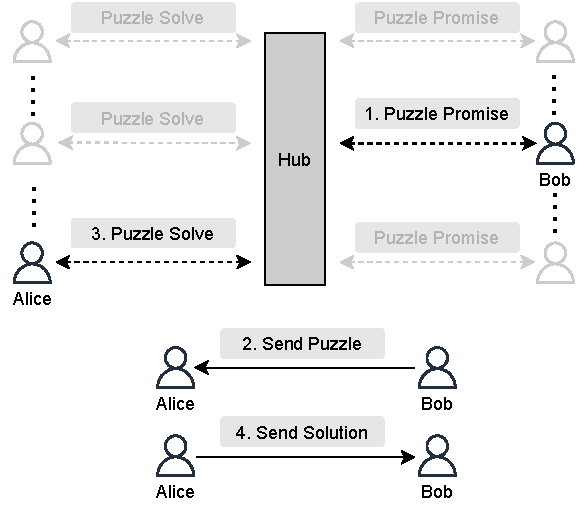
\includegraphics[width=0.7\linewidth]{syncpuzzle.pdf}
    \caption{Protocol flow of a synchronization puzzle, the underlying cryptographic mechanism of Tumblebit and \AAL, which we formalize as Blind Conditional Signatures.
    Dotted double-edged arrows indicate 2-party protocols. Solid arrows indicate secure point-to-point communication.}
    \label{fig:syncpuzzle_overview}
  \end{figure}

One line of work, initiated by TumbleBit~\cite{NDSS:HABSG17}, uses a protocol paradigm which we refer to as a \emph{synchronization puzzle}. A synchronization puzzle is a three-party protocol between a sender Alice, a mixer Hub, and a recipient Bob (\Cref{fig:syncpuzzle_overview}). Synchronization puzzle protocols consist of four steps: (1) Hub and Bob execute the \emph{puzzle promise} phase with respect to some message $m_{HB}$, which outputs a puzzle $\tau$ containing a hidden signature $\sigma_{HB}$ on $m_{HB}$. (2) Bob sends $\tau$ to Alice via a private channel, who (3) uses it to execute the \emph{puzzle solver} phase with Hub with respect to another message $m_{AH}$. At the end of this phase, Alice obtains the signature $\sigma_{HB}$ on $m_{HB}$ and Hub learns $\sigma_{AH}$ on $m_{AH}$. To conclude, (4) Alice sends $\sigma_{HB}$ to Bob. A synchronization puzzle protocol should satisfy the following properties:
\begin{itemize}
    \item \textbf{Blindness}: In the puzzle solver phase, Hub \emph{blindly} helps solve $\tau$, i.e., the phase should not reveal anything about $\tau$ to Hub. (This keeps Alice and Bob unlinkable from the point of view of Hub.)
    \item \textbf{Unlockability}: If the puzzle solver phase completes successfully, $s$ must be a valid secret for $\tau$. (This ensures that the Hub cannot learn $\sigma_{AH}$ without revealing $\sigma_{HB}$.)
    \item \textbf{Unforgeability}: Bob cannot output a valid signature $\sigma_{HB}$ on $m_{HB}$ before the puzzle solver phase completes. (This ensures Bob cannot learn $\sigma_{HB}$ without Hub learning $\sigma_{AH}$.)
\end{itemize}
To use a synchronization puzzle to realize an atomic payment, the parties set $m_{AH} : (A \xrightarrow{c+\epsilon} H)$ and $m_{HB} : (H \xrightarrow{c} B)$, where $(U_i \xrightarrow{c} U_j)$ denotes a payment of $c$ coins from user $U_i$ to $U_j$. Then $\sigma_{AH}$ and $\sigma_{HB}$ are set to the signatures authorizing $m_{AH}$ and $m_{HB}$, respectively. Thus, at the completion of the protocol Alice will have sent $c$ coins to Bob (and paid a fee of $\epsilon$ to Hub).

% Tumblebit realizes a synchronization puzzle via RSA encryption~\cite{RSA78} and hashed timelock contract (HTLCs), the latter of which is only present in certain ``scripting'' cryptocurrencies (e.g., Bitcoin and Ethereum).
% \noemi{RSA is used to encrypt the puzzle solution, and the ciphertext is rerandomized by Alice as in A2L. The HTLCs are used to extract the secret once the signature posted; A2L substitutes this with adaptor signatures.}

\subsubsection{Anonymous Atomic Locks (\texorpdfstring{\AAL}{A2L})}

A follow-up work~\cite{SP:TaiMorMaf21} introduces Anonymous Atomic Locks (\AAL), a protocol for off-chain coin mixing which requires only limited capabilities of the underlying blockchain, i.e., no scripting functionality.
Before we describe its approach to instantiating synchronization puzzles, we introduce the notion of \emph{adaptor signatures}, which will be used as a building block:

\begin{definition}[adaptor signature~\cite{AC:AEEFHM21}]
    An adaptor signature scheme $\Pi_\ADP := (\kgen, \presign, \prevrfy, \adapt, \vrfy, \ext)$ is defined with respect to a digital signature scheme $\Pi_\DS$ and an NP relation $\Rel$:
    \begin{description}
        \item[$\kgen(\secparam) \to (\vk, \sk)$:] The key generation algorithm is the same as in the underlying digital signature scheme, i.e., $\Pi_\DS.\kgen$.
        \item[$\presign(\sk, m, Y) \to \presig$:] The pre-signing algorithm takes as input a signing key $\sk$, message $m$, and instance $Y$ of the relation $\Rel$ and returns a pre-signature $\presig$.
        \item[$\prevrfy(\vk, m, Y, \presig) \to \{0, 1\}$:] The pre-verification algorithm checks that a pre-signature is well-formed.
        \item[$\adapt(\presig, y) \to \sigma$:] Given a witness $y$ for the instance $Y$, this algorithm adapts the pre-signature $\presig$ into a valid signature $\sigma$.
        \item[$\vrfy(\vk, m, \sigma) \to \{0, 1\}$:] The verification algorithm is the same as in the underlying digital signature scheme, i.e., $\Pi_\DS.\vrfy$.
        \item[$\ext(\presig, \sigma, Y) \to y$:] Given a pre-signature $\presig$ and a signature $\sigma$ generated with respect to some instance $Y$, the extract algorithm outputs the corresponding witness $y$ such that $(Y, y) \in \Rel$.
    \end{description}
\end{definition}

An adaptor signature scheme should satisfy the following properties: \emph{pre-signature correctness}, which guarantees that for all instances $Y \in \Lang_\Rel$ and honestly generated $\presig, \sigma$, the pre-signature and signature pass (pre-)verification and the extracted witness $y' \gets \ext(\presig, \sigma, Y)$ should satisfy $(Y, y') \in \Rel$; \emph{unforgeability}, which is a straightforward extension of the standard existential unforgeability notion (EUF-CMA) for digital signatures; \emph{pre-signature adaptability}, which states that for any $Y \in \Lang_\Rel$ and corresponding pre-signature $\presig$, pre-verification implies that $\presig$ can be adapted to a verifying signature $\sigma$; and \emph{witness extractability}, which says that it is difficult for an adversary to adapt an honestly-generated pre-signature $\presig$ into a signature $\sigma$ which verifies but where $y' \gets \ext(\presig, \sigma, Y)$ such that $(Y, y') \notin \Lang_\Rel$. We refer the reader to \cite{CCS:GMMMTT22} for formal definitions.

Anonymous Atomic Locks (\AAL)~\cite{SP:TaiMorMaf21} uses a rerandomizable CPA-secure encryption scheme $\Pi_\ENC$ and an adaptor signature scheme $\Pi_\ADP$ to realize a synchronization puzzle which is compatible with a wider range of cryptocurrencies. Specifically, the puzzle promise phase outputs to Bob a ciphertext $c \gets \Pi_\ENC.\enc(\ek_H, y)$ and a pre-signature $\presig_{HB}$ on $m_{HB}$ with respect to a discrete-log instance $Y := g^y$. Bob sends $(c, Y)$ to Alice, who rerandomizes them using fresh randomness $r$ to $(c', Y') := (\Pi_\ENC.\enc(\ek_H, y+r), g^y g^r)$. She can now use $Y'$ to produce a pre-signature $\presig_{AH}$ on $m_{AH}$ and executes the puzzle solver phase with Hub using $c', \presig_{AH}$. Hub can use $\sk_H$ to decrypt $c'$ and obtain $y' := y+r$, which it uses to complete the presignature into a full signature $\sigma_{AH}$ on $m_{AH}$ (thus completing the left side of the payment). This allows Alice to extract $y'$ via $\Pi_\ADP.\ext(\presig_{AH}, \sigma_{AH}, Y')$ and use her knowledge of $r$ to recover $y$, which she sends to Bob. Now Bob uses $y$ to adapt $\presig_{HB}$ to a full signature $\sigma_{HB}$ on $m_{HB}$, thereby completing the right side of the payment.

\cite{SP:TaiMorMaf21} defines an ideal functionality, which is reproduced as $\F_\BCS$ in \cite{CCS:GMMMTT22}, and gives a UC proof of security for \AAL:

\begin{theorem}[Main theorem~\cite{SP:TaiMorMaf21} (paraphrased)\footnote{As we will show, this theorem is incorrect.}]\label{thm:a2l}
    Let $\sf COM$ be a secure commitment scheme, $\NIZK$ be a non-interactive zero-knowledge proof, $\Pi_\DS$ be EUF-CMA-secure signature schemes, $\Rel$ be an NP-relation, $\Pi_\ADP$ be a secure adaptor signature scheme with respect to $\Pi_\DS$ and $\Rel$, and $\Pi_\ENC$ be a rerandomizable CPA-secure encryption scheme. Then \AAL UC-realizes the ideal functionality $\F_\BCS$ assuming anonymous guaranteed delivery channels and a synchronous network.
\end{theorem}

\subsubsection{Insecurity of \texorpdfstring{\AAL}{A2L}}\label{sec:a2l-attacks}

In \cite{CCS:GMMMTT22}, we analyzed the \AAL protocol~\cite{SP:TaiMorMaf21} and found that, in contrast to its claims, it is not secure. Although \AAL was proven secure in the universal composability (UC)~\cite{FOCS:Canetti01} framework, we show that a gap in their formal model allows two constructions which are completely insecure despite meeting their definitions: one admits a key recovery attack and the other allows a colluding sender and recipient to steal coins from the mixer. We will show how to close this gap in \Cref{sec:bcs}.

In more detail, we show that there exist cryptographic primitives which satisfy the prerequisites of \AAL's main theorem, but allow \textit{(a)} a \emph{key recovery attack}, in which a malicious user is able to learn the long-term secret of the hub or \textit{(b)} a \emph{one-more signature attack}, in which a sender and recipient can collude to obtain $\secpar+1$ tokens from the hub while only sending $\secpar$ tokens. Both attacks run in polynomial time and succeed with overwhelming probability. These instantiations of \AAL are specifically crafted to allow an attack and do not imply that all instantiations of \AAL are broken; however, we cannot prove the security of \AAL either. This tension is discussed further in \Cref{sec:bcs}.

Below we give informal descriptions of both attacks. We refer the reader to \cite{CCS:GMMMTT22} for detailed descriptions and analysis. Both attacks rely on the fact that in the \AAL protocol, Hub offers a malicious Alice something very close to a decryption oracle. This oracle, which we refer to as $\oaal$, is programmed with a decryption key $\dk$ and takes as input a verification key $\vk$, message $m$, group element $h$, ciphertext $c$, and pre-signature $\presig$. It computes the plaintext $\tilde{x} \gets \Pi_\ENC.\dec(\dk, c)$ and attempts to use it to adapt $\presig$, i.e., computes $\sigma' \gets \Pi_\ADP.\adapt(\presig, \tilde{x})$. If it is successful, i.e., $\Pi_\ADP.\vrfy(\vk, m, \sigma') = 1$ or equivalently $\tilde{x} = x$, it returns $\sigma'$; otherwise it returns $\perp$. Note that the sender (Alice) can easily generate inputs to query the oracle: $\vk$ is the querier's own verification key, $m$ can be any arbitrary message in the message space, and generating $\presig$ that is valid when adapted with the (unknown) value $x$ requires only knowledge of the party's own signing key and a value $h = g^x$. The counterexamples below make use of the fact that $\sigma'$ implicitly reveals $\tilde{x} = \Pi_\ADP.\ext(\presig, \sigma, h)$. This leakage is not addressed in \AAL's proof of security.

\paragraph{Key recovery attack.} We show how to recover Hub's decryption key $\dk$ with $\secpar$ queries to $\oaal$ when \AAL is instantiated with an encryption scheme $\Pi_\ENC$ which, in addition to being re-randomizable and CPA-secure (as required by \Cref{thm:a2l}) has the following properties:
\begin{itemize}
    \item linearly homomorphic over $\ZZ_p$
    \item circular secure for bit encryption, i.e., CPA-secure even given the bitwise encryption of the decryption key
    \item the aforementioned ciphertexts $(c_1, \dots, c_\secpar) := (\enc(\ek, \dk_1), \dots, \enc(\ek,\allowbreak \dk_\secpar))$ are included in the encryption key $\ek$
\end{itemize}

Note that even with these additional assumptions, $\Pi_\ENC$ still satisfies the conditions of \Cref{thm:a2l}, and yet \AAL instantiated with such a scheme is insecure. In particular, a malicious Alice can use $\secpar$ queries to recover Hub's long-term decryption key $\dk$. The intuition of the attack is as follows: Alice samples a witness $x \sample \ZZ_p$ and computes the ciphertext $c \gets \Pi_\ENC.\enc(\ek, x)$. Now she can use the provided bitwise encryption of $\dk$ to homomorphically compute $c_i' := \Pi_\ENC.\enc(\ek, x + \dk_i)$ for each bit of the key. Getting the remaining inputs to the oracle is easy, since she can use her signing key to compute $h := g^x$ and $\presig \gets \Pi_\ADP.\presign(\sk, m, h)$ for an arbitrary $m$. At this point, she can query $\oaal(\vk_A, m, h, c_i, \presig)$ for $i = 1, \dots, \secpar$. The oracle returns $\perp$ if and only if $\dk_i = 1$, since $g^{x+1} \neq h = g^x$; otherwise, the oracle outputs an adapted signature $\sigma'$, and Alice learns that $\dk_i = 0$. This attack succeeds with probability 1. Recall that obtaining a non-$\perp$ response from the oracle is equivalent to authorizing a payment of $c$ coins from Alice to Hub, so it costs $nc \leq n\secpar$ coins (where $n$ is the number of 0 bits in $\dk$).

\paragraph{One-more signature attack.} Next, we show how to steal 1 coin from the hub for every $q \in O(\secpar)$ successful payments, i.e., learn $q+1$ signature witnesses for every $q$ non-$\perp$ queries to $\oaal$. This attack works when \AAL is instantiated with an encryption scheme $\Pi_\ENC$ which, in addition to being re-randomizable and CPA-secure (as required by \Cref{thm:a2l}) has the following properties:
\begin{itemize}
    \item linearly homomorphic over $\ZZ_p$
    \item supports homomorphic evaluation of the \emph{conditional bit flip} ($\sf CFlip$) function, defined as $\Pi_\ENC.\mathsf{CFlip}(\ek, i, \Pi_\ENC.\enc(\ek, x)) := \Pi_\ENC.\enc(\ek, y)$ where
    \[
        y = \begin{cases} 
            x &\text{ if } x[i] = 0\\ 
            x \oplus e_i &\text{ if } x[i] = 1
        \end{cases}
    \]
    Here $e_i$ is the $i$th unit vector and $x[i]$ is the $i$th bit of $x$.
\end{itemize}
Again, even with these additional assumptions, $\Pi_\ENC$ still satisfies the conditions of \Cref{thm:a2l}, and yet \AAL instantiated with such a scheme is insecure. The intuition of the attack is as follows: given $q+1$ puzzle promise instances $(c_j := \Pi_\ENC.\enc(\ek, x_j), h_j := g^{x_j})$ for $j = 1, \dots, q+1$, Alice will attempt to learn the bits of $x_1$ by conditionally flipping them one at a time. Each query $i$ consists of a ciphertext $c'$ containing a random linear combination of the $c_j$'s, where $c_1$'s $i$th bit is also conditionally flipped, and $h'$ which is the same random linear combination of $h_j$'s \emph{without} $x_1$'s $i$th bit being conditionally flipped. If the oracle response is $\perp$, $c'$ and $h'$ were inconsistent which means the $i$th bit of $x_1$ was a 1. Otherwise, if the oracle responds with a non-$\perp$ value $y_i$, the $i$th bit of $x_1$ was a 0 and Alice has additionally learned the value of one random linear combination of the $x_j$'s. By the time $q = \sizeof{x_1}$ non-$\perp$ queries have been made, Alice has learned all the bits of $x_1$ and also has $\secpar$ linear equations with $\secpar$ unknowns. Since the coefficients are uniformly chosen, the equations are, with all but negligible probability, linearly independent; and since $\ZZ_p$ is a field, the solution is uniquely determined and can be found efficiently via Gaussian elimination. Furthermore, the length of each $x_i$ is $\secpar$, so the attack is efficient.

\subsubsection{Formalizing Blind Conditional Signatures}\label{sec:bcs}

In light of our attacks, the natural question is whether we can establish formally rigorous security guarantees for an (appropriately patched) \AAL protocol. While it seems unlikely that \AAL can achieve UC-security (more discussion on this later), we investigate whether it satisfies some weaker, but still meaningful, notion of security. Our main observation here is that a weak notion of CCA-security for encryption schemes suffices to provide formal guarantees for \AAL. This notion, which we refer to as \emph{one-more CCA-security}, (roughly) states that it is hard to recover the plaintexts of $n$ ciphertexts while querying a decryption oracle at most $n-1$ times. Importantly, this notion is, in principle, not in conflict with the homomorphism/re-randomization requirements, contrary to standard CCA-security.

To place the synchronization puzzle on firmer foundations, in \cite{CCS:GMMMTT22} we introduce a new primitive called blind conditional signatures (BCS)\footnote{not to be confused with conditional blind signatures~\cite{EPRINT:ZacGroPag17}.} which captures the core synchronization puzzle functionality. We give game-based security definitions for BCS and show how to modify \AAL to obtain a new protocol, \AALplus, which meets these definitions. We also give a UC-secure construction of BCS, dubbed \AALUC, which requires much more complex machinery. In this section, we summarize the remaining contributions and constructions of~\cite{CCS:GMMMTT22}. 

\paragraph{Game-based definitions.} Towards establishing a formal analysis of \AAL, we introduce the notion of blind conditional signatures (BCS) which captures the core synchronization puzzle functionality. We propose game-based definitions similar in spirit to the well-established security definitions of regular blind signatures~\cite{C:Chaum82,JC:SchUnr17}. 

\begin{definition}[Blind Conditional Signature]
    A blind conditional signature $\Pi_\mathsf{BCS}\allowbreak :=(\setup, \Promise, \Pay, \Open)$ is defined with respect to a signature scheme $\Pi_\DS := (\kgen,\sign,\vrfy)$ and consists of the following efficient algorithms.
    
    \begin{itemize}%[leftmargin=*]
    \item {$(\tilde{\ek}, \tilde{\dk})\gets \setup(\secparam)$}: The setup algorithm takes as input the security parameter $\secparam$ and outputs a key pair $(\tilde{\ek}, \tilde{\dk})$.
    \item {$(\bot, \{\tau, \bot\}) \gets \Promise \left\langle \begin{matrix} H \left(\tilde{\dk}, \sk^H, m_{HB} \right)\\ B \left(\tilde{\ek}, \vk^H, m_{HB} \right) \end{matrix} \right\rangle $}: The puzzle promise algorithm is an interactive protocol between two users $H$ (with inputs the decryption key $\tilde{\dk}$, the signing key $\sk^H$, and a message $m_{HB}$) and $B$ (with inputs the encryption key $\tilde{\ek}$, the verification key $\vk^H$, and a message $m_{HB}$)  and returns $\bot$ to $H$ and either a puzzle $\tau$ or $\bot$ to $B$.
    \item {$(\{(\sigma^*, s), \bot\}, \{\sigma^*, \bot\}) \gets \Pay \left\langle \begin{matrix} A \left(\sk^A, \tilde{\ek}, m_{AH}, \tau\right)\\ H \left(\tilde{\dk}, \vk^A, m_{AH} \right) \end{matrix} \right\rangle $}: The puzzle solving algorithm is an interactive protocol between two users $A$ (with inputs the signing key $\sk^A$, the encryption key $\tilde{\ek}$, a message $m_{AH}$, and a puzzle $\tau$) and $H$ (with inputs the decryption key $\tilde \dk$, the verification key $\vk^A$, and a message $m_{AH}$) and returns to both users either a signature $\sigma^*$ ($A$ additionally receives a secret $s$) or $\bot$.
    \item {$\{\sigma, \bot\}\gets \Open(\tau, s)$}: The open algorithm takes as input a puzzle $\tau$ and a secret $s$ and returns a signature $\sigma$ or $\bot$.
    \end{itemize}
\end{definition}

Informally, correctness holds if for all honest executions of the protocols, the resulting signatures $\sigma$ and $\sigma^*$ verify.

% Next, we define correctness.
% \begin{definition}[Correctness]
%     A blind conditional signature $\Pi_\mathsf{BCS}$ is correct if for all $\secpar\in \mathbb{N}$, all $(\tilde{\ek}, \tilde{\dk})$ in the support of $\setup(\secparam)$, all $(\vk^H, \sk^H)$ and $(\vk^A, \sk^A)$ in the support of $\Pi_\DS.\kgen(\secparam)$, and all pairs of messages $(m_{HB}, m_{AH})$, it holds that
%     $$
%     \Pr\left[\vrfy(\vk^H,m_{HB}, \Open(\tau, s)) = 1\right] = 1
%     $$
%     and
%     $$
%     \Pr\left[\vrfy(\vk^A,m_{AH}, \sigma^*) = 1\right] = 1
%     $$
%     where 
%     \begin{itemize}%[leftmargin=*]
%         \item $\tau \gets \Promise \left\langle \begin{matrix} H \left(\tilde{\dk}, \sk^H, m_{HB} \right)\\ B \left(\tilde{\ek}, \vk^H, m_{HB}\right) \end{matrix} \right\rangle$ and
%         \item $((\sigma^*, s), \sigma^*) \gets \Pay \left\langle \begin{matrix} A \left(\sk^A,  \tilde{\ek}, m_{AH}, \tau\right)\\ H \left(\tilde{\dk}, \vk^A, m_{AH}\right) \end{matrix} \right\rangle$.
%     \end{itemize}
% \end{definition}
%

The game-based security guarantees of BCS consist of three properties:
\begin{description}
    \item[Blindness.] Our definition of blindness is akin to the strong blindness notion of standard blind signatures~\cite{C:Chaum82}, in which the adversary picks the keys (as opposed to the weak version in which they are chosen by the experiment)\footnote{We opt for this stronger version since we want to provide anonymity even in the case of a fully malicious hub, which can pick its keys adversarially to try to link a sender/receiver pair.}. Roughly speaking, it says that two promise/solve sessions cannot be linked together by the hub.\footnote{We do not consider the case in which Hub colludes with either Alice or Bob, since deanonymization is trivial (Alice (resp. Bob) simply reveals the identity of Bob (resp. Alice) to Hub); this is in line with \cite{SP:TaiMorMaf21}.}\footnote{In previous works, descriptions of unlinkability assume an explicit step for blinding the puzzle $\tau$ between $\Promise$ and $\Pay$. Here, we assume that $\Pay$ performs this blinding functionality.}
    % \begin{definition}[Blindness]
    %     A blind conditional signature $\Pi_\BCS$ is blind if there exists a negligible function $\negl$ such that for all $\secpar \in \NN$ and all PPT adversaries $\adv$, the following holds:
    %     \[ \prob{\expUnlink^{\adv}_{\Pi_{\mathsf{puzzle}}}(\secpar) = 1} \le \frac{1}{2} + \negl\]
    %     where $\expUnlink$ is defined in~\cref{fig:exp_unlinkability}.\footnote{In previous works, descriptions of unlinkability assume an explicit step for blinding the puzzle $\tau$ between $\Promise$ and $\Pay$. Here, we assume that $\Pay$ performs this blinding functionality.}
    % \end{definition}
    \item[Unlockability.] This property says that it should be hard for Hub to create a valid signature on Alice's message that does not allow Bob to unlock the full signature in the corresponding promise session.
    % \begin{definition}[Unlockability]
    %     A blind conditional signature $\Pi_\mathsf{BCS}$ is unlockable if there exists a negligible function $\negl$ such that for all $\secpar \in \NN$ and all PPT adversaries $\adv$, the following holds:
    %     \[ \prob{\expUnlock^{\adv}_{\Pi_{\mathsf{BCS}}}(\secpar) = 1} \le \negl\]
    %     where $\expUnlock$ is defined in~\cref{fig:exp_unlockability}.
    % \end{definition}
    \item[Unforgeability.] Our definition of unforgeability is inspired by the unforgeability of blind signatures~\cite{C:Chaum82}. We require that Alice and Bob cannot recover $q$ signatures from Hub while successfully querying the solving oracle at most $q-1$ times. Since each successful query reveals a signature from Alice's key (which in turn corresponds to a transaction from Alice to Hub), this requirement implicitly captures the fact that Alice and Bob cannot steal coins from Hub. The winning condition $b_0$ captures the scenario where the adversary forges a signature of the hub on a message previously not used in any promise oracle query.
    The remaining conditions $b_1, b_2$ and $b_3$ together capture the scenario in which the adversary outputs $q$ valid distinct key-message-signature tuples while having queried for solve only $q-1$ times. Hence, in the second condition, the attacker manages to \emph{complete} $q$ promise interactions with only $q-1$ solve interactions, whereas in the first winning condition, the adversary computes a \emph{fresh} signature that is not the completion of any promise interaction. These conditions are technically incomparable: an attacker that succeeds under one condition does not imply an attacker succeeding on the other.
    It is important to note that this is different from the unforgeability notion of blind signatures (where the attacker only has access to a single signing oracle), since in our case the hub is offering the attacker two oracles: promise and solve.
    % \begin{definition}[Unforgeability]
    % A blind conditional signature $\Pi_\mathsf{BCS}$ is \emph{unforgeable} if there exists a negligible function $\negl$ such that for all $\secpar \in \NN$ and all PPT adversaries $\adv$, the following holds:
    % \begin{equation*}
    %      \prob{\expSec^{\adv}_{\Pi_{\mathsf{BCS}}}(\secpar) = 1} \le \negl
    % \end{equation*}
    % where $\expSec$ is defined in~\cref{fig:exp_security_ab}.
    % \end{definition}
\end{description}

%     \begin{figure}
        \centering
        \makebox[0pt]{\begin{minipage}{1.35\textwidth}
        \begin{pchstack}[boxed]
        \begin{pcvstack}
        %%%%%%%%%%%%%%%%%%%%%%%%%%%%%%%%%%%%%
        %%%%% Blindness (unlinkability) %%%%%
        %%%%%%%%%%%%%%%%%%%%%%%%%%%%%%%%%%%%%
        \begin{pchstack}%[boxed]
        \procedure[space=auto,codesize=\small]{Blindness experiment $\expUnlink^{\adv}_{\Pi_{\mathsf{BCS}}}(\secpar)$}{
        \hfill\\[-0.5\baselineskip]
       (\tilde{\ek}, \vk^H_0, \vk^H_1, (m_{HB,0}, m_{AH,0}), (m_{HB,1}, m_{AH,1})) \gets \adv(\secparam)\\
        (\vk_0^A, \sk_0^A) \gets \kgen(\secparam)\\
        (\vk_1^A, \sk_1^A) \gets \kgen(\secparam)\\
        \tau_0 \gets \Promise \left\langle  \adv(\vk_0^A, \vk_1^A), \bob(\tilde{\ek}, \vk^H_0, m_{HB,0}) \right\rangle\\
        \tau_1 \gets \Promise \left\langle  \adv(\vk_0^A, \vk_1^A), \bob(\tilde{\ek}, \vk^H_1, m_{HB,1}) \right\rangle\\
        b \gets \{0,1\}\\
        (\sigma^*_0, s_0) \gets \Pay \left\langle  \alice \left(\sk_0^A, \tilde{\ek}, m_{AH,0}, \tau_{0 \oplus b}\right), \adv \right\rangle \\
        (\sigma^*_1, s_1) \gets \Pay \left\langle  \alice \left(\sk_1^A, \tilde{\ek}, m_{AH,1}, \tau_{1 \oplus b}\right), \adv \right\rangle \\
        \mathbf{if~}(\sigma^*_0 = \bot) \lor (\sigma^*_1 = \bot) \lor (\tau_0 = \bot) \lor (\tau_1 = \bot)\\
        \quad \sigma_0 := \sigma_1 := \bot\\
        \mathbf{else}\\
        \quad \sigma_{0 \oplus b} \gets \Open(\tau_{0 \oplus b}, s_0)\\
        \quad \sigma_{1 \oplus b} \gets \Open(\tau_{1 \oplus b}, s_1)\\
        b' \gets \adv(\sigma_0, \sigma_1)\\
        \mathbf{return}\ (b = b')
        }
        \end{pchstack}
        \pcvspace
        %%%%%%%%%%%%%%%%%%%%%%%%%%%%%%%%%%%%%
        %%%%%      Unlockability        %%%%%
        %%%%%%%%%%%%%%%%%%%%%%%%%%%%%%%%%%%%%
        \begin{pchstack}%[boxed]
        \procedure[space=auto,codesize=\small]{Unlockability experiment $\expUnlock^{\adv}_{\Pi_{\mathsf{BCS}}}(\secpar)$}{
        \hfill\\[-0.5\baselineskip]
        (\tilde{\ek}, \vk^H, m_{HB}, m_{AH}) \gets \adv(\secparam)\\
        (\vk^A, \sk^A) \gets \kgen(\secparam)\\
        \tau \gets \Promise \left\langle  \adv(\vk^A), \bob(\tilde{\ek}, \vk^H, m_{HB}) \right\rangle\\
        \textbf{if } \tau = \bot\\
        \quad (\hat{\sigma}, \hat{m}) \gets \adv\\ 
        \quad b_0 := (\vrfy(\vk^A,\hat{\sigma}, \hat{m}) =1)\\
        \textbf{if } \tau \neq \bot\\
            \quad (\sigma^*,s) \gets \Pay \left\langle  \alice \left(\sk^A, \tilde{\ek}, m_{AH},\tau\right), \adv \right\rangle\\
        \quad (\hat{\sigma}, \hat{m}) \gets \adv\\ 
        \quad b_1 := (\vrfy(\vk^A,\hat{\sigma}, \hat{m}) =1) \land (\hat{m} \neq m_{AH})\\
         \quad b_2 := (\vrfy(\vk^A,\sigma^*, m_{AH}) =1)\\
        \quad b_3 := (\vrfy(\vk^H, m_{HB}, \Open(\tau,s)) \neq1) \\
         \mathbf{return}\ b_0 \lor b_1 \lor (b_2 \land b_3)
        }
        \end{pchstack}
        \end{pcvstack}
        \pchspace
        %%%%%%%%%%%%%%%%%%%%%%%%%%%%%%%%%%%%%
        %%%%%      Unforgeability       %%%%%
        %%%%%%%%%%%%%%%%%%%%%%%%%%%%%%%%%%%%%
        \begin{pchstack}%[boxed]
        \begin{pcvstack}
        \procedure[space=auto,codesize=\small]{Unforgeability experiment $\expSec^{\adv}_{\Pi_{\mathsf{BCS}}}(\secpar)$}{
        \hfill\\[-0.5\baselineskip]
    \mathcal{L} := \emptyset, Q := 0 \\
    (\tilde{\ek}, \tilde{\dk}) \gets \setup(\secparam)\\
    (\vk_1^H, m_1, \sigma_1), \ldots, (\vk_q^H, m_q, \sigma_q)  \gets \adv^{\oracle\mathsf{PP}(\cdot), \oracle\mathsf{PS}(\cdot)}(\tilde{\ek})\\
    b_0 := \exists i \in [q] \suchthat (\vk_i^H,\cdot) \in \mathcal{L} \land (\vk_i^H,m_i) \notin \mathcal{L} \\
    \qquad \qquad  \land \vrfy(\vk_i^H,m_i,\sigma_i) = 1\\
    b_1 := \forall i \in [q], (\vk_i^H,m_i) \in \mathcal{L} \land \vrfy(\vk_i^H, m_i, \sigma_i) = 1\\
    b_2 := \bigwedge_{i,j \in [q], i \ne j}  (\vk_i^H, m_i, \sigma_i) \ne (\vk_j^H, m_j, \sigma_j) \\
    b_3 := (Q \le q-1) \\
    \mathbf{return}\ b_0 \lor (b_1 \land b_2 \land b_3)
    }
    \pcvspace
    
    \procedure[space=auto,codesize=\small]{$\oracle\mathsf{PP}(m)$}{
    \hfill\\[-0.5\baselineskip]
    (\vk^H, \sk^H) \gets \Pi_\ADP.\kgen(\secparam)\\
    \mathcal{L} := \mathcal{L} \cup \{ (\vk^H,m) \}\\
    \bot \gets \Promise\langle H(\tilde{\dk}, \sk^H, m), \adv(\vk^H) \rangle \\
    }
    
    
    \procedure[space=auto,codesize=\small]{$\oracle\mathsf{PS}(\vk^A, m')$}{
    \hfill\\[-0.5\baselineskip]
    \sigma^* \gets \Pay\langle \adv, H(\tilde{\dk}, \vk^A, m') \rangle \\
    \mathbf{if}\ \sigma^* \ne \bot\ \mathbf{then}~ Q:= Q+ 1
    }
        \end{pcvstack}
    \end{pchstack}
    \end{pchstack}
    \end{minipage}}
    \caption{BCS security games \label{fig:bcs_games}}
    \end{figure}
%
    % \begin{figure}
    %     \centering
    %     \begin{pchstack}[boxed]
    %     \procedure[space=auto,codesize=\small]{$\expUnlock^{\adv}_{\Pi_{\mathsf{BCS}}}(\secpar)$}{
    %     \hfill\\[-0.5\baselineskip]
    %     (\tilde{\ek}, \vk^H, m_{HB}, m_{AH}) \gets \adv(\secparam)\\
    %     (\vk^A, \sk^A) \gets \kgen(\secparam)\\
    %     \tau \gets \Promise \left\langle  \adv(\vk^A), \bob(\tilde{\ek}, \vk^H, m_{HB}) \right\rangle\\
    %     \textbf{if } \tau = \bot\\
    %     \quad (\hat{\sigma}, \hat{m}) \gets \adv\\ 
    %     \quad b_0 := (\vrfy(\vk^A,\hat{\sigma}, \hat{m}) =1)\\
    %     \textbf{if } \tau \neq \bot\\
    %         \quad (\sigma^*,s) \gets \Pay \left\langle  \alice \left(\sk^A, \tilde{\ek}, m_{AH},\tau\right), \adv \right\rangle\\
    %     \quad (\hat{\sigma}, \hat{m}) \gets \adv\\ 
    %     \quad b_1 := (\vrfy(\vk^A,\hat{\sigma}, \hat{m}) =1) \land (\hat{m} \neq m_{AH})\\
    %      \quad b_2 := (\vrfy(\vk^A,\sigma^*, m_{AH}) =1)\\
    %     \quad b_3 := (\vrfy(\vk^H, m_{HB}, \Open(\tau,s)) \neq1) \\
    %      \mathbf{return}\ b_0 \lor b_1 \lor (b_2 \land b_3)
    %     }
    % \end{pchstack}
    %     \caption{Unlockability experiment} 
    %     \label{fig:exp_unlockability}
    % \end{figure}
    % %
    % \begin{figure}
    %     \centering
    %     \begin{pchstack}[boxed]
    %     \begin{pcvstack}
    %     \procedure[space=auto,codesize=\small]{$\expSec^{\adv}_{\Pi_{\mathsf{BCS}}}(\secpar)$}{
    %     \hfill\\[-0.5\baselineskip]
    % \mathcal{L} := \emptyset, Q := 0 \\
    % (\tilde{\ek}, \tilde{\dk}) \gets \setup(\secparam)\\
    % (\vk_1^H, m_1, \sigma_1), \ldots, (\vk_q^H, m_q, \sigma_q)  \gets \adv^{\oracle\mathsf{PP}(\cdot), \oracle\mathsf{PS}(\cdot)}(\tilde{\ek})\\
    % b_0 := \exists i \in [q] \suchthat (\vk_i^H,\cdot) \in \mathcal{L} \land (\vk_i^H,m_i) \notin \mathcal{L} \\
    % \qquad \qquad  \land \vrfy(\vk_i^H,m_i,\sigma_i) = 1\\
    % b_1 := \forall i \in [q], (\vk_i^H,m_i) \in \mathcal{L} \land \vrfy(\vk_i^H, m_i, \sigma_i) = 1\\
    % b_2 := \bigwedge_{i,j \in [q], i \ne j}  (\vk_i^H, m_i, \sigma_i) \ne (\vk_j^H, m_j, \sigma_j) \\
    % b_3 := (Q \le q-1) \\
    % \mathbf{return}\ b_0 \lor (b_1 \land b_2 \land b_3)
    % }
    % \pcvspace
    
    % \procedure[space=auto,codesize=\small]{$\oracle\mathsf{PP}(m)$}{
    % \hfill\\[-0.5\baselineskip]
    % (\vk^H, \sk^H) \gets \Pi_\ADP.\kgen(\secparam)\\
    % \mathcal{L} := \mathcal{L} \cup \{ (\vk^H,m) \}\\
    % \bot \gets \Promise\langle H(\tilde{\dk}, \sk^H, m), \adv(\vk^H) \rangle \\
    % }
    
    
    % \procedure[space=auto,codesize=\small]{$\oracle\mathsf{PS}(\vk^A, m')$}{
    % \hfill\\[-0.5\baselineskip]
    % \sigma^* \gets \Pay\langle \adv, H(\tilde{\dk}, \vk^A, m') \rangle \\
    % \mathbf{if}\ \sigma^* \ne \bot\ \mathbf{then}~ Q:= Q+ 1
    % }
    %     \end{pcvstack}
    % \end{pchstack}
    %     \caption{Unforgeability experiment}
    %     \label{fig:exp_security_ab}
    % \end{figure}
    

% The security games are given in \Cref{fig:bcs_games}. We define security as the collection of all three properties:
We refer the reader to \cite{CCS:GMMMTT22} for the security games. Security is defined as the collection of all three properties:

\begin{definition}[Security]
    A blind conditional signature $\Pi_\mathsf{BCS}$ is secure if it is blind, unlockable, and unforgeable. %, i.e., if there exist negligible functions $\negln{1}, \negln{2}, \negln{3}$ such that for all $\secpar \in \NN$ and all PPT adversaries $\adv$, all of the following hold:
    % \begin{align*}
    %     \prob{\expUnlink^{\adv}_{\Pi_{\mathsf{puzzle}}}(\secpar) = 1} &\le \frac{1}{2} + \neglnf{1}\\
    %     \prob{\expUnlock^{\adv}_{\Pi_{\mathsf{BCS}}}(\secpar) = 1} &\le \neglnf{2}\\
    %     \prob{\expSec^{\adv}_{\Pi_{\mathsf{BCS}}}(\secpar) = 1} &\le \neglnf{3}
    % \end{align*}
\end{definition}    

\paragraph{The \AALplus protocol: a secure version of \AAL.}
With the BCS formalism in place, we can prove that an appropriately modified version of \AAL, which we call \AALplus, satisfies the above definitions. Our analysis comes with an important caveat: we analyze the security of our scheme in the \emph{linear-only encryption model}. This is a model introduced by Groth~\cite{TCC:Groth04} that only models adversaries that are restricted to perform ``legal'' operations on ciphertexts, similarly to the generic/algebraic group model. While this is far from a complete analysis, it increases our confidence in the security of the system.\footnote{We resort to the LOE model because of the seemingly inherent conflict between linear homomorphism and CCA-like security, both of which are needed for our application (in our setting, the adversary has access to something akin to a decryption oracle). Indeed, even proving that ElGamal encryption is CCA1-secure in the standard model is a long-standing open problem, and we believe that the \AAL approach would inherently hit this barrier without some additional assumption. \noemi{Recent work~\cite{EC:Schage24} resolves this open question by giving an impossibility result for the CCA1-security of ElGamal.}} We defer the details of the \AALplus protocol, its analysis, and a discussion of its overhead with respect to \AAL to \cite{CCS:GMMMTT22}.

% \newcommand{\blue}[1]{\textcolor{blue}{#1}}
\newcommand{\green}[1]{\textcolor{teal}{#1}}
\newcommand{\twoPC}{\ensuremath{\mathsf{2PC}}}

\begin{figure*}%[!t]
\centering
%\resizebox{\textwidth}{!}{
\makebox[0pt]{\begin{minipage}{1.4\textwidth}
%%%%%%%%%%%%%%%%%%%%%%%%%%%%%%%%%
%%%%%%    PUZZLE PROMISE    %%%%%
%%%%%%%%%%%%%%%%%%%%%%%%%%%%%%%%%
\begin{pchstack}[boxed]
    \procedure{Public parameters: group description $(\GG, g, q)$, message $m_{HB}$}{
 	\text{ $\Promise \langle H( \dk_H, \sk_{HB}^H), \cdot \rangle$} \< \< \text{$\Promise \langle \cdot, B(\ek_H, \vk_{HB}^H) \rangle$} \\[][\hline]
	\pcln s \sample \ZZ_p, Y := g^s \< \< \\ [-0.15\baselineskip][]
	\pcln c \gets \Pi_\ENC.\enc(\ek_H, s) \< \< \\ [-0.15\baselineskip][]
	\pcln \pi_s \gets \NIZK.\prove( (\ek_H, Y, c), s)  \< \< \\ [-0.15\baselineskip][]
	\pcln \tilde{\sigma}_{HB}^H \gets \Pi_\ADP.\presig( \sk_{HB}^H, m_{HB}, Y ) \< \< \\ [-0.85\baselineskip][]
	\pcln \< \sendmessageright*{Y, c, \pi_s, \tilde{\sigma}_{HB}^H}\< \\ [-0.55\baselineskip][]
	\pcln \< \< {\mathbf{If}\ \NIZK.\vrfy((\ek_H,Y,c), \pi_s) \neq 1\ \mathbf{ then}\ \pcreturn \bot} \\ [-0.15\baselineskip][]
	\pcln \< \< \mathbf{If}\ \Pi_\ADP.\prevrfy(\vk_{HB}^H, m_{HB}, Y, \tilde{\sigma}_{HB}^H) \neq 1\ \mathbf{then} \\ [-0.15\baselineskip][]
	\pcln \< \< \quad \pcreturn \bot \\ [-0.15\baselineskip][]
	\pcln \< \< \mathbf{set}\ \tau := (m_{HB}, \tilde{\sigma}_{HB}^H, (Y, c)) \\ [-0.15\baselineskip][]
	\pcln \pcreturn \bot \< \< \pcreturn \tau
}
\end{pchstack}
%%%%%%%%%%%%%%%%%%%%%%%%%%%%%%%%%
%%%%%%     PUZZLE SOLVER    %%%%%
%%%%%%%%%%%%%%%%%%%%%%%%%%%%%%%%%
\begin{pchstack}[boxed]
    \procedure{Public parameters: group description $(\GG, g, q)$, message $m_{AH}$}{ 
 	\text{$\Pay \langle A(\sk_{AH}^A, \ek_H, \tau), \cdot\rangle$} \< \< \text{$\Pay \langle \cdot, H(\dk_H, \vk_{AH}^A) \rangle$} \\[][\hline]
 	\pcln \pcparse \tau := ( \cdot, \cdot, (Y, c)) \< \< \\ [-0.15\baselineskip][]
 	\pcln r \sample \ZZ_p, Y' := Y \cdot g^r \< \< \\ [-0.15\baselineskip][]
 	\pcln \tilde{\sigma}_{AH}^A \gets \Pi_\ADP.\presig( \sk_{AH}^A, m_{AH}, Y') \< \< \\ [-0.85\baselineskip][] 
 	\pcln \< \sendmessageright*{Y', \tilde{\sigma}_{AH}^A} \< \\ [-0.55\baselineskip][]
 	\pcln \< \< \mathbf{If}\ \Pi_\ADP.\prevrfy(\vk_{AH}^A, m_{AH}, Y', \tilde{\sigma}_{AH}^A) \neq 1\ \mathbf{then} \\ [-0.15\baselineskip][]
 	\< \< \quad \pcreturn \bot\\ [-0.15\baselineskip][]
 	\pcln \< \begin{subprocedure}
 	\dbox{\procedure[linenumbering]{$\twoPC((r,c), (\dk_H))$}{
 	\pcif \ek_H \neq \Pi_\ENC.\mathsf{Gen}(\dk_H)\\
 	\pcthen \text{abort}\\
 	s^* \gets \Pi_\ENC.\dec(\dk_H, c)\\
 	z := s^* + r\\
 	\pcreturn ((\bot), (z))
 	}}
 	\end{subprocedure}
 	\< \\ [-0.15\baselineskip][]
 	\pcln \< \< \mathbf{If}\ Y' \neq g^z\ \mathbf{then}\ \pcreturn \bot\\ [-0.15\baselineskip][]
 	\pcln \< \< \sigma_{AH}^A \gets \Pi_\ADP.\adapt(\tilde{\sigma}_{AH}^A, z)\\ [-0.85\baselineskip][]
 	%\pcln \< \< \sigma_{AH}^H \gets \Pi_\sign(\sk_{AH}^H, m)\\ [-0.85\baselineskip][]
 	\pcln \< \sendmessageleft*{{\sigma}_{AH}^A} \< \\ [-0.55\baselineskip][]
 	\pcln \mathbf{If}\ \Pi_\ADP.\vrfy(\vk_{AH}^A, m_{AH}, \sigma_{AH}^A) \neq 1\ \mathbf{then} \< \< \\ [-0.15\baselineskip][]
 	\pcln \quad \pcreturn \bot \< \< \\ [-0.15\baselineskip][]
 	\pcln z' \gets \Pi_\ADP.\ext(\tilde{\sigma}_{AH}^A, \sigma_{AH}^A, Y')\< \< \\ [-0.15\baselineskip][]
 	\pcln s := z'-r \< \< \\ [-0.15\baselineskip][]
 	\pcln \pcreturn (\sigma_{AH}^A, s) \< \< \pcreturn \sigma_{AH}^A
}
\end{pchstack}
%%%%%%%%%%%%%%%%%%%%%%%%%%%%%%%%%
%%%%%%     SETUP & OPEN     %%%%%
%%%%%%%%%%%%%%%%%%%%%%%%%%%%%%%%%
\begin{center}
    \begin{pchstack}[boxed]
        \procedure[space=auto,codesize=\small]{$\setup(\secparam)$}{
    (\ek_H, \dk_H) \gets \Pi_\ENC.\kgen(\secparam)\\
    \pcreturn (\ek_H, \dk_H)
    }
    
    \pchspace
    
    \procedure[space=auto,codesize=\small]{$\open(\tau, s)$}{
    \mathbf{parse}\ \tau := ( \cdot, \tilde{\sigma}, \cdot)\\
    \sigma \gets \Pi_\ADP.\adapt(\tilde \sigma, s)\\
    \pcreturn \sigma
    }
    \end{pchstack}
\end{center}
\end{minipage}}
%}
\caption{Puzzle promise, puzzle solver, and open protocols of \AALUC}
\label{fig:a2l_uc}
\end{figure*}

% \begin{figure}
%     \centering
%     \begin{pchstack}[boxed]
%         \procedure[space=auto,codesize=\small]{$\setup(\secparam)$}{
%     (\ek_H, \dk_H) \gets \Pi_\ENC.\kgen(\secparam)\\
%     \mathbf{set}\ \tilde \pk := \ek_H, \tilde \sk := \dk_H\\
%     \pcreturn (\tilde \pk, \tilde \sk)
%     }
    
%     \pchspace
    
%     \procedure[space=auto,codesize=\small]{$\open(\tau, s)$}{
%     \mathbf{parse}\ \tau := ( \cdot, \tilde{\sigma}, \cdot)\\
%     \sigma \gets \Pi_\ADP.\adapt(\tilde \sigma, s)\\
%     \pcreturn \sigma
%     }
%     \end{pchstack}
%     \caption{Setup and Open algorithms of our conditional puzzle construction}
%     \label{fig:our_protocol_algorithms}
% \end{figure}

% \begin{figure*}[h]
% \centering
% %\resizebox{\textwidth}{!}{
% \begin{pchstack}[boxed]
%     \procedure{Public parameters: group description $(\GG, g, q)$, message $m_{HB}$}{ 
%  	\text{ $\Promise \langle H( \dk_H, \sk_{HB}^H), \cdot \rangle$} \< \< \text{$\Promise \langle \cdot, B(\ek_H, \vk_{HB}^H) \rangle$} \\[][\hline]
% 	\pcln s \sample \ZZ_p, Y := g^s \< \< \\ [-0.15\baselineskip][]
% 	\pcln c \gets \Pi_\ENC.\enc(\ek_H, s) \< \< \\ [-0.15\baselineskip][]
% 	\pcln \pi_s \gets \NIZK.\prove( (\ek_H, Y, c), s)  \< \< \\ [-0.15\baselineskip][]
% 	\pcln \tilde{\sigma}_{HB}^H \gets \Pi_\ADP.\presig( \sk_{HB}^H, m_{HB}, Y ) \< \< \\ [-0.85\baselineskip][]
% 	\pcln \< \sendmessageright*{Y, c, \pi_s, \tilde{\sigma}_{HB}^H}\< \\ [-0.55\baselineskip][]
% 	\pcln \< \< {\mathbf{If}\ \NIZK.\vrfy((\ek_H,Y,c), \pi_s) \neq 1\ \mathbf{ then}\ \pcreturn \bot} \\ [-0.15\baselineskip][]
% 	\pcln \< \< \mathbf{If}\ \Pi_\ADP.\prevrfy(\vk_{HB}^H, m_{HB}, Y, \tilde{\sigma}_{HB}^H) \neq 1\ \mathbf{then} \\ [-0.15\baselineskip][]
% 	\pcln \< \< \quad \pcreturn \bot \\ [-0.15\baselineskip][]
% 	\pcln \< \< \mathbf{set}\ \tau := (m_{HB}, \tilde{\sigma}_{HB}^H, (Y, c)) \\ [-0.15\baselineskip][]
% 	\pcln \pcreturn \bot \< \< \pcreturn \tau
% % 	\pcln \< \< \text{If } \NIZK.\vrfy(\pi_s, (Y,c)) \neq 1 \text{ then abort} \\ [-0.15\baselineskip][]
% % 	\pcln \< \< \pcsend\ (Y, c)\ \pcto\ A \\ [-0.15\baselineskip][]
% % 	\pcln \< \< \pcreceive\ s^*\ \pcfrom\ A \\ [-0.15\baselineskip][]
% % 	\pcln \< \< \sigma_{HB}^H \gets \Pi_\ADP.\adapt(\tilde{\sigma}_{HB}^H, s^*) \\ [-0.15\baselineskip][]
% % 	\pcln \< \< \sigma_{HB}^B \gets \Pi_\DS.\sign(\sk_{HB}^B, m_{HB}) \\ [-0.15\baselineskip][]
% % 	\pcln \< \< \pcpost\ (m_{HB}, [\sigma_{HB}^H, \sigma_{HB}^B])\ \pcto\ \BB\\ [-0.15\baselineskip][]
% % 	\pcln \pcreturn \top \< \< \pcreturn \top 
% }
% \end{pchstack}
% %}
% \vspace{-0.2cm}
% \caption{Puzzle promise protocol of \sysnameuc}
% \label{fig:our_protocol_hub_bob}
% \vspace{-0.4cm}
% \end{figure*}

% \begin{figure*}
% \centering
% %\resizebox{\textwidth}{!}{
% \begin{pchstack}[boxed]
%     \procedure{Public parameters: group description $(\GG, g, q)$, message $m_{AH}$}{ 
%  	\text{$\Pay \langle A(\sk_{AH}^A, \ek_H, \tau), \cdot\rangle$} \< \< \text{$\Pay \langle \cdot, H(\dk_H, \vk_{AH}^A) \rangle$} \\[][\hline]
%  	\pcln \pcparse \tau := ( \cdot, \cdot, (Y, c)) \< \< \\ [-0.15\baselineskip][]
%  	\pcln r \sample \ZZ_p, Y' := Y \cdot g^r \< \< \\ [-0.15\baselineskip][]
%  	\pcln \tilde{\sigma}_{AH}^A \gets \Pi_\ADP.\presig( \sk_{AH}^A, m_{AH}, Y') \< \< \\ [-0.85\baselineskip][] 
%  	\pcln \< \sendmessageright*{Y', \tilde{\sigma}_{AH}^A} \< \\ [-0.55\baselineskip][]
%  	\pcln \< \< \mathbf{If}\ \Pi_\ADP.\prevrfy(\vk_{AH}^A, m_{AH}, Y', \tilde{\sigma}_{AH}^A) \neq 1\ \mathbf{then} \\ [-0.15\baselineskip][]
%  	\< \< \quad \pcreturn \bot\\ [-0.15\baselineskip][]
%  	\pcln \< \begin{subprocedure}
%  	\dbox{\procedure[linenumbering]{$\twoPC((r,c), (\dk_H))$}{
%  	\pcif \ek_H \neq \Pi_\ENC.\mathsf{Gen}(\dk_H)\\
%  	\pcthen \text{abort}\\
%  	s^* \gets \Pi_\ENC.\dec(\dk_H, c)\\
%  	z := s^* + r\\
%  	\pcreturn ((\bot), (z))
%  	}}
%  	\end{subprocedure}
%  	\< \\ [-0.15\baselineskip][]
%  	\pcln \< \< \mathbf{If}\ Y' \neq g^z\ \mathbf{then}\ \pcreturn \bot\\ [-0.15\baselineskip][]
%  	\pcln \< \< \sigma_{AH}^A \gets \Pi_\ADP.\adapt(\tilde{\sigma}_{AH}^A, z)\\ [-0.85\baselineskip][]
%  	%\pcln \< \< \sigma_{AH}^H \gets \Pi_\sign(\sk_{AH}^H, m)\\ [-0.85\baselineskip][]
%  	\pcln \< \sendmessageleft*{{\sigma}_{AH}^A} \< \\ [-0.55\baselineskip][]
%  	\pcln \mathbf{If}\ \Pi_\ADP.\vrfy(\vk_{AH}^A, m_{AH}, \sigma_{AH}^A) \neq 1\ \mathbf{then} \< \< \\ [-0.15\baselineskip][]
%  	\pcln \quad \pcreturn \bot \< \< \\ [-0.15\baselineskip][]
%  	\pcln z' \gets \Pi_\ADP.\ext(\tilde{\sigma}_{AH}^A, \sigma_{AH}^A, Y')\< \< \\ [-0.15\baselineskip][]
%  	\pcln s := z'-r \< \< \\ [-0.15\baselineskip][]
%  	\pcln \pcreturn (\sigma_{AH}^A, s) \< \< \pcreturn \sigma_{AH}^A
% }
% \end{pchstack}
% %}
% \vspace{-0.2cm}
% \caption{Puzzle solver protocol of \sysnameuc}
% \label{fig:our_protocol_alice_hub}
% \vspace{-0.4cm}
% \end{figure*}

\paragraph{UC-security.} The next question that we set out to answer is whether we can construct a synchronization puzzle that satisfies the strong notion of UC-security. We do not know how to prove that \AAL (or \AALplus) is secure under composition, which is why we prove \AALplus secure only in the game-based setting. The technical difficulty in proving UC-security is that blindness is unconditional, and we lack a ``trapdoor mechanism'' that allows the simulator to link adversarial sessions during simulation in the security analysis; the proof of UC-security in \cite{SP:TaiMorMaf21} is flawed due to this same reason. 

Thus, we develop a different protocol, called \AALUC %and presented in \Cref{fig:a2l_uc}, 
that we can prove realizes the BCS UC functionality $\Fbcs$ (essentially the same functionality introduced in \cite{SP:TaiMorMaf21}) in the standard model. We assume the following cryptographic building blocks:
\begin{itemize}
    \item An adaptor signature scheme $\Pi_\ADP$ defined with respect to $\Pi_\DS$ and a hard relation $R_\mathsf{DL}$.
    \item A UC-secure NIZK proof system $\Pi_\NIZK$ for the language $$\mathcal{L} := \{ (\ek, Y,c) \mid \exists s, \suchthat c \gets \Pi_\ENC.\enc(\ek, s) \land Y = g^s \}. $$ 
    \item A UC-secure 2PC protocol.
    \item A CCA-secure~\cite{FOCS:BDJR97} encryption scheme $\Pi_\ENC := (\kgen, \enc, \dec)$ with unique decryption keys, i.e., $\ek$ can be computed injectively from $\dk$.
\end{itemize}

\AALUC uses the heavy hammer of multi-party computation to reconcile the need for both CCA-security and rerandomizability of the encryption scheme. As in \AAL and \AALplus, the puzzle sent in the puzzle promise phase consists of a (now CCA-secure) encryption $c$ of the witness $y$ and the instance $Y := g^y$ along with a pre-signature $\presig_{HB}$; but in the puzzle solver phase, Alice can only rerandomize the instance on her own to obtain $Y' := Y \cdot g^r$, which she uses for the pre-signature $\presig_{AH}$. To rerandomize the witness contained in $c$, Alice and Hub engage in a two-party computation (2PC) protocol in which Alice inputs $r, c$ and Hub inputs its decryption key. The 2PC decrypts $c$ and adds $r$ to the result, which it outputs to Hub. The rest of the protocol continues as before: Hub uses the rerandomized witness to complete $\presig_{AH}$ to $\sigma_{AH}$, Alice extracts the witness, derandomizes it, and sends it to Bob, and Bob uses it to complete $\presig_{HB}$ to $\sigma_{HB}$. The details of the protocol, the ideal functionality $\Fbcs$, and the UC security proof are left to \cite{CCS:GMMMTT22}.

Because the scheme relies on standard general-purpose cryptographic tools such as a UC-secure 2PC, it incurs a significant increase in computation costs. We stress that we view this scheme as a proof-of-concept, and leave further improvements for practical efficiency as an open problem.  We hope that the scheme will shed some light on the barriers that need to be overcome in order to construct a practically efficient UC-secure synchronization puzzle.
\section{The Cicada Framework}\label{sec:cicada_framework}

We present Cicada, our framework for non-interactive private auctions/elections, in \Cref{fig:cicada}. Cicada can be applied to voting and auction schemes where the scoring function $\Score = f \circ t$ has a linear tally function $t$. The framework uses a linear HTLP (\Cref{sec:tlp}), vector packing scheme (\Cref{sec:packing}), and matching NIZK (\Cref{sec:sigmas}) to ensure correctness of submissions by proving both the well-formedness of the puzzle and the solution's membership in $\X$.

At a high level, Cicada enables auction or voting schemes with the following five steps. 
\emph{First}, system participants agree on a delay parameter $\Ttime$ and packing parameter $\ell$. The $\Setup$ algorithm outputs HTLP public parameters $\pparam$ (note this might require private randomness) and initializes a set of the tally HTLPs $\mathcal{Z}$ containing zeros. 
\emph{Second}, a user $i$ uses the $\Seal$ algorithm to encode their submission (a bid or ballot) $\vec{v}_i$ into (a set of) HTLP(s) $\Z_i$. $\Seal$ also outputs a NIZK $\pi_i$ proving that the submission $\Z_i$ is well-formed, i.e., is in the domain $\mathcal{X}$ of the scoring function $\Score$. Users will send these submissions and corresponding proofs to the on-chain coordinator. 
\emph{Third}, the coordinator (Cicada smart contract) runs $\Aggr$ to verify the user-submitted proof $\pi_i$, and if it is valid, aggregate the user submission $\Z_i$ into the tally HTLPs $\Z$, resulting in updated tally HTLP(s) $\Z'$. 
\emph{Fourth}, after the voting/bidding period has ended, any party can open the tally HTLPs $\Z$ off-chain by running $\Open$, which outputs the opening(s) $\mathcal{S}$ of the tally HTLP(s) $\Z$ along with a proof of correct opening $\pi_{\textsf{open}}$ (using a proof of solution $\pos$, see \Cref{sec:sigmas}). The off-chain solver will send $\mathcal{S}, \pi_{\mathsf{open}}$ to the contract. 
\emph{Fifth}, the on-chain contract runs $\Finalize$ to verify the correctness of $\mathcal{S}$ by checking $\pi_{\mathsf{open}}$. If the check passes, it computes the auction/election winner(s) as $y=f(\vec{v})$.

% \noemi{In Cicada we need to talk about the function that is applied to the final tally, not the ballots -- maybe we could introduce a definition of ``linear'' protocols $\Sigma : \X^n \to \Y$ which are those functions that have an associated function $\Sigma_{\sf winner}: \X' \to \Y$ such that $\Sigma_{\sf winner}(t) = \Sigma(s_1, \dots, s_n)$ where $t = f(s_1, \dots, s_n)$ for some linear function $f$.}
%\noemi{difference between $\Sigma$ and $\Sigma_{\sf winner}$ is the domain, $\X^n$ and $\X$, resp.}

Intuitively, submission privacy follows from the security of the HTLP and zero-knowledge of the NIZK used: the submission can't be opened before time $\Ttime$ and none of the proofs leak any information about it. Non-malleability is enforced by requiring the NIZK to be a proof of knowledge and including the user's identity $i$ in the instance to prove, e.g., including it in the hash input of the Fiat-Shamir transform. This prevents a malicious actor from replaying a different user's ballot correctness proof.
% \istvan{Correctness is due to the correctness of the underlying NIZKs. Submission privacy is reduced to the HTLP sequentiality, while non-malleability is ensured by the proof of knowledge property of our applied NIZKs.} 

\begin{figure*}[t!]
\begin{mdframed}
\begin{center}
    \textbf{The Cicada Framework}
\end{center}
Let $\Sigma: \X^n \rightarrow \Y$ be the scoring function of a voting/auction scheme
where $\Score = f \circ t$ for a linear function $t$ and
% $\Sigma = f \circ g$ for some linear function $g$ and 
$\X = [0,w]^m$. 
Let $\htlp$ a linear HTLP, $\Ttime \in \NN$ a time parameter representing the election/auction length, and $(\PSetup, \pack, \unpack)$ a packing scheme.
Let $\NIZK$ be a NIZKPoK for 
submission correctness (language depends on $\Sigma, \htlp$; see \Cref{sec:sigmas})
% the language $\{(i, Z) : \exists x \text{ s.t. } Z \in {\sf Im}(\htlp.{\sf Gen}(\pack(x))) \land\ x \in \X\}$ 
and \pos\ be a proof of correct HTLP solution (see \Cref{sec:sigmas}). 

\hrulefill %%%%%%%%%%%%%%%%%%%%%%%%%%%%%%
\begin{description}
    \item[$\Setup(\secparam, \Ttime, \ell) \randout (\pp, \Z)$.] 
    Set up the public parameters $\pp_{\NIZK} \sample \NIZK.\Setup(\secparam)$, $\pp_{\sf tlp} \sample \htlp.\Setup(\secparam, \Ttime)$, and $\pp_{\sf pack} \gets \PSetup(\ell, w)$. 
    Let $\Z = \{Z_j\}_{j \in [m/\ell]}$ where $Z_j \sample \htlp.{\sf Gen}(0)$. Output $\pp := (\pp_{\sf tlp}, \pp_{\sf pack}, \pp_\NIZK)$ and $\Z$.
    \item[$\Seal(\pp,i, \vec{v}_i) \randout (\Z_i, \pi_i)$.] Parse $\vec{v}_i := \vec{v}_{i,1} || \dots || \vec{v}_{i,m/\ell}$. Compute $Z_{i,j} \gets \htlp.{\sf Gen}(\pack(\vec{v}_{i,j}))~\forall j \in [m/\ell]$ and $\pi_i \gets \NIZK.\prove((i, \Z_i), \vec{v}_i)$.
    % $s_{i,j} \gets \pack(\vec{v}_{i,j})$ for all $j \in [m/\ell]$. 
    Output $(\Z_i := \{Z_{i,j}\}_{j \in [m/\ell]}, \pi_i)$ 
    \item[$\Aggr(\pp,\Z,i,\Z_i,\pi_i) \rightarrow \Z'$.] If $\NIZK.\vrfy((i, \Z_i), \pi_i) = 1$, update $\Z$ to $\Z \boxplus \Z_i$. %, where $\boxplus$ is applied pairwise to elements of $\Z,\Z_i$.
    \item[$\Open(\pp,\Z) \rightarrow (\mathcal{S}, \pi_{\sf open})$.] Parse $\Z := \{Z_j\}_{j \in [m/\ell]}$ and solve for the encoded tally $\mathcal{S} = \{s_j\}_{j \in [m/\ell]}$ where $s_j \gets \htlp.{\sf Solve}(Z_j)$. Prove the correctness of the solution(s) as $\pi_{\sf open} \gets \pos.{\sf Prove}(\mathcal{S}, \Z, 2^\Ttime)$ and output $(\mathcal{S}, \pi_{\sf open})$.
    \item[$\Finalize(\pp, \Z, \mathcal{S}, \pi_{\sf open}) \rightarrow \{y,\perp\}$.] If $\pos.{\sf Verify}(\mathcal{S}, \Z, 2^\Ttime, \pi_{\sf open}) \neq 1$, return $\perp$. Otherwise, parse $S := \{s_j\}_{j \in [m/\ell]}$ and let $\Vec{v} := \vec{v}_1 || \dots || \vec{v}_{m/\ell}$, where $\vec{v}_j \gets \unpack(s_j)~\forall j \in [m/\ell]$. Output 
    % $y = f(\vec{v})$.
    $y$ such that $y = \Sigma(\vec{v})$.
\end{description}
\end{mdframed}
\caption{The Cicada framework for non-interactive private auctions and elections.}
\label{fig:cicada}
\end{figure*}

As we will see next, this captures many common schemes such as cumulative voting and sealed-bid auctions. 
Cicada introduces a crucial design choice via the packing parameter $\ell\in[m]$, which defines a storage-computation trade-off that we detail in~\Cref{sec:implementation}. %The on-chain footprint of a protocol is minimized by using a ballot correctness proof system $\sf NIZK$ with low verification cost. % this seems kind of obvious? And if anything it belongs in the implementation section

% \section{Application to voting schemes}\label{sec:voting}

% \todo{revisit this} The main reason we are interested in building protocols for cardinal voting schemes is that they allow voters to express more fine-grained preferences. Put differently, they bypass Arrow's impossibility theorem~\cite{arrow1950difficulty}, i.e., cardinal voting schemes satisfy non-dictatorship, unrestricted domain, independence of irrelevant alternatives and Pareto efficient. 

\paragraph{Additive voting.}
Many common voting schemes are ``additive'', meaning each ballot (a length-$m$ vector) is simply added to the tally, and a finalization function $f$ is applied to the tally after the voting phase has ended to determine the winner. 
Additive voting schemes include first-past-the-post (FPTP), approval, range, and cumulative voting. Simple ranked-choice voting schemes, e.g., Borda count~\cite{Emerson13}, are also additive, differing only in what qualifies as a ``proper'' ballot (restrictions on vector entry domain, vector norm, etc.; see \Cref{tab:voting_schemes}). 
Thus, we can use Cicada to instantiate private voting protocols for all these schemes.

% \paragraph{Majority vote and approval voting.}
% We start off by describing a protocol for approval voting. Approval voting is a generalization of majority vote, whereby, a voter can cast a vote for multiple candidates. In case of a majority vote, a ballot can be thought of as a binary vector of Hamming weight $1$, while approval voting lifts this restriction, i.e., the ballot can be any length-$m$ binary vector $\vec{b} \in\{0,1\}^{m}$. The challenge is to design a protocol that applies a single HTLP for tallying the approval votes.

% Following~\cite{hirt2000efficient}, we encode the $i$th voter's ballot as the integer
% \begin{equation}\label{eq:approval_voting_ballot_encoding}
%     % b_j\in \Big\{
%     % \sum\limits_{i=1}^{m} b_j^{(i)} (n+1)^{i-1}: b_j^{(i)} = 1 \iff\textit{j votes for candidate i}\in[m]\Big\}. 
%     b_i\in \Big\{
%     \sum\limits_{j=1}^{m} b_i^{(j)} (n+1)^{j-1}: b_i^{(j)} = 1 \iff\textit{i votes for candidate j}\in[m]\Big\}. 
% \end{equation}
% Note the number of votes for candidate $j$ can be obtained as $\sum\limits^{n}_{i=1}b_i\bmod{(n+1)^{j-1}}$.

% \begin{figure}[h!]
% \begin{mdframed}
% \begin{description}
%     \item[$\mathsf{Setup}(\secparam, \Ttime) \randout (\pparam, Z^*)$.]  Set up HTLP parameters $\pparam_{\sf tlp} \sample \htlp.\Setup(\secparam, \Ttime)$. Let $Z^* \sample \htlp.{\sf Gen}(\pparam_{\sf tlp}, 0)$. Output $\pparam := (\pparam_{\sf tlp},Z^*)$.
%     \item[$\Seal(\pparam,i,b_i) \randout (Z_i, \pi_{\sf i})$.] Let $b_i$ encode the $i$th user's approval vote as in Equation~\ref{eq:approval_voting_ballot_encoding}. Let $Z_i \gets \htlp.{\sf Gen}(\pparam_{\sf tlp}, b_i)$. The  correctness proof $\pi_i$ is obtained as $\pi_i:=\bigwedge\limits_{i=1}^{m}\zkprove(\mathcal{R}_{\pokemon}(Z_i/Z'_j,0,n^{j-1};b_i) \lor\mathcal{R}_{\pokemon}(Z_i/Z'_j,1,n^{j-1};b_i))$, where $Z'_j$ is the residual approval vote, i.e., $Z'_j\gets\htlp.{\sf Gen}(\pparam_{\sf tlp}, b_i\mod{n^{j-1}})$. 
    
%     Output $(Z_i,\pi_i)$.
%     \item[$\Aggr(\pparam,Z^*,Z_j,\pi_{\sf j}) \rightarrow Z^*$.] If $\zkvfy((\pparam,j,Z_j),\pi_{\sf j}) \neq 1$, leave $Z^*$ unchanged and abort. Otherwise, update $Z^* = Z^* \oplus Z_j$.
%     \item[$\Open(\pparam,Z^*,\mathcal{R}) \rightarrow s^*$.] Solve the tally puzzle for $s^* \gets \htlp.{\sf Solve}(\pparam_{\sf tlp}, Z^*)$.
%     \item[$\Finalize(\pparam, s^*) \rightarrow {\sf winner}$.] Compute the sum of the votes for each candidate $j \in [m]$ as $s^*_j := s^* \mod{n^{j-1}}$. The winner is $\argmax_j \{s^*_1, \dots, s^*_m\}$.
% \end{description}


% \end{mdframed}
% \caption{A protocol for approval voting among $m$ candidates using a single HTLP.}
% \label{fig:voting_approval}
% \end{figure}

% \paragraph{Ranked choice voting, range voting, and cumulative voting.}

% In a na\"ive Borda count protocol, the tally consists of $m$ HTLPs $\{Z^{*}_i\}^{m}_{i=1}$ (one per candidate) that encode the accumulated points of each candidate, initially set to $0$.  During the voting phase, each voter creates $m$ HTLPs $\{Z_i\}^{m}_{i=1}$ encoding integers from $0$ to $m-1$. Afterwards, voters homomorphically add each ballot HTLP $Z_i$ to the corresponding tally HTLP $Z^{*}_i$. This solution is suboptimal in terms of the number of HTLPs needed. 
% 
% We show a protocol that requires only a single HTLP. Let the $i$th voter's preference vector be defined as $\mathbf{q^{(i)}}=(q^{(i)}_1,q^{(i)}_2,\dots,q^{(i)}_m)$, which is required to be a permutation of $[0,m-1]$ .
% % $\forall j:q^{(i)}_j\in[0,m-1]\land\forall j,k: q^{(i)}_{j}\neq q^{(i)}_k$ i.e., it is a permutation of $[0,m-1]$. 
% % Let $\mathbf{p}=(p_1,p_2,\dots,p_m)$ be a vector of prime numbers such that $\min_{i}p_i\geq (m-1)n$ and $\prod\limits_{i=1}^{m} p_i\leq N$.
% Now encode $\vec{q}^{(i)}$ as an integer $s_i$ using the Chinese Remainder Theorem (see \cref{sec:packing}) and encode it in an HTLP $Z_i$.
% % Specifically, $s_i\equiv q^{(i)}_{j}\mod{p_j}$, which can be efficiently found by the Chinese Remainder's Theorem (CRT).
% The user submits their puzzle $Z_i$ with the accompanying zero-knowledge proofs for ballot correctness, and the on-chain contract homomorphically adds $Z_i$ and $Z^*$.

% At the end of the voting phase, a single party solves the tally HTLP $Z^*$ to obtain the solution $s^{*}$. We claim that the total preference points (Borda counts) for candidate $j$ can be computed as $s^{*}\mod{p_j}$. The correctness of this protocol for ranked voting follows from the observation that for any preference $j$, we have 
% \begin{equation}\label{eq:borda_correctness_argument}
%     s^{*}\bmod{p_j}=\sum\limits^n_{i=1}s_i\bmod{p_j}\equiv\sum\limits^n_{i=1}q^{(i)}_j\bmod{p_j}=\sum\limits^n_{i=1}q^{(i)}_j\leq(m-1)n. 
% \end{equation}

\begin{theorem}\label{thm:cicada}
    Given a linear scoring function $\Sigma$, a secure NIZKPoK $\NIZK$ and proof of solution $\pos$, a secure $\htlp$, and a packing scheme $({\sf PSetup},\allowbreak \pack,\allowbreak \unpack)$, the Cicada protocol $\Pi_\Sigma$ (\Cref{fig:cicada}) is a secure time-locked voting/auction protocol. % i.e., it satisfies correctness, bid/ballot privacy, and non-malleability.
\end{theorem}

% We delegate the full proof to \Cref{sec:secproofs}.
\begin{proof}
\def\Exp{\ensuremath{\mathsf{ExpSPriv}_{\Pi_\Sigma}^\adv(\secpar,\Ttime,i)}}
    For simplicity, we give a proof for the simple case of $\X=[0,1]$, i.e., submissions consist of a single bit, but our argument generalizes to larger domains $\X$. Let $n \in \mathbb{N}$ be the number of users.

    The correctness of the Cicada framework (cf.~\Cref{def:correctness_cicada}) follows by construction and from the correctness of the underlying building blocks (i.e., soundness in the case of the proof systems).
    
    Next, we prove submission privacy.
    Let $\Exp$ be the original submission privacy game for the Cicada scheme $\Pi_\Sigma$ with $\Ttime$-bounded adversary $\adv$, cf.~\Cref{def:submission_privacy}. We define a series of hybrids to show that 
    \[ 
        \Pr[\Exp = 1] \leq \negl 
    \]
    for all $\secpar,\Ttime \in \mathbb{N}$ and $i\in[n]$.
    
    \underline{$\hybrid_0$:} This is the original game $\Exp$, where $Z_i \gets \htlp.{\sf Gen}(b)$ and $\pi_i \gets \NIZK.\prove(i, Z_i, b)$.
    
    \underline{$\hybrid_1$:} Replace $\pi$ with $\tilde{\pi} \gets {\sf NIZK}.\Sim(i, Z_i)$. $\hybrid_1$ is indistinguishable from $\hybrid_0$ by the zero-knowledge property of $\sf NIZK$.

    \underline{$\hybrid_2$:} Replace $Z_i$ with $Y_i \gets \htlp.{\sf Gen}(1-b)$ and $\tilde{\pi}$ with $\tilde{\sigma} \gets {\sf NIZK}.\Sim(i, Y_i)$. $\hybrid_1$ and $\hybrid_2$ are indistinguishable because the distributions $\{Z_i, \Sim(i, Z_i)\}$ and $\{Y_i, \Sim(i, Y_i)\}$ are indistinguishable since $\{Z_i\}, \{Y_i\}$ are indistinguishable by the security of $\htlp$.

    % \underline{$\hybrid_3$:} Replace $\tilde{\pi}$ with $\tilde{\sigma} \gets {\sf NIZK}.\Sim(i, Y_i)$. $\hybrid_3$ is indistinguishable from $\hybrid_2$ again by security of $\htlp$: since the distributions of $Z_i, Y_i$ are indistinguishable, so must the distributions ...
    
    \underline{$\hybrid_3$:} Replace $\tilde{\sigma}$ with $\sigma \gets \NIZK.\prove(i, Y_i, 1-b)$. $\hybrid_3$ is indistinguishable from $\hybrid_2$ by the zero-knowledge property of $\sf NIZK$.

    This series of hybrids implies $\Pr[b'=b] \approx_\secpar \Pr[b'=1-b]$, where $b'$ is the output of $\adv$ in $\hybrid_0$ or $\hybrid_3$, respectively. Therefore $\Pr[\Exp = 1] \leq \frac{1}{2} + \negl[\secpar]$.
    
    % --- reduction attempt ---
    % Suppose towards a contradiction that there exists a $\Ttime$-bounded adversary $\adv$ who wins the submission privacy game with non-negligible probability. We will use give a $\Ttime$-bounded adversary $\bdv$ capable of violating either the zero-knowledge of $\sf NIZK$ or the privacy of $\htlp$.

    % Given a puzzle $Z$ containing an unknown bit $b_1$ and a proof $\pi$ that some independent unknown bit $b_2 \in [0,1]$, $\bdv$ constructs two different queries $(Z, \tilde{\pi})$ and $(\tilde{Z}, \pi)$ as follows: sample $i \sample [n]$ and compute $\tilde{\pi} \gets {\sf NIZK}.\Sim(i, Z)$ and $\tilde{Z} \gets \htlp.{\sf Gen}(0)$. Query $\adv$ on both 

    Finally, we show that if $\NIZK$ is a PoK and $\htlp$ is secure, then Cicada is non-malleable, cf.~\Cref{def:non_malleability}. Suppose towards a contradiction that Cicada is malleable. We will use this and the fact that $\NIZK$ is a PoK to construct an adversary $\bdv$ which has non-negligible advantage in the $\htlp$ security game. Again, we work in the simple case $\X = [0,1]$, i.e., $m,\ell,w=1$, but the argument generalizes to other parameter settings.
    
    Since by our assumption Cicada is malleable, there exists $\adv$ which outputs $(i, \cdot, \Z_i, \pi_i) \notin \mathcal{Q}$ such that $\NIZK.\vrfy((i,\allowbreak \Z_i), \pi)=1$ with non-negligible probability. 
    % Also, $\sf NIZK$ is a PoK, so it has an efficient knowledge extractor $\Ext$. 
    Given a puzzle $Z_b$ containing some unknown bit $b$, $\bdv$ works as follows. First, it computes $(\pparam, Z) \sample \Setup(\secparam, \Ttime, 1)$ and sends them to the non-malleability adversary $\adv$. $\bdv$ responds to $\adv$'s oracle queries $(j, b_j)$ with honestly computed $(Z_j, \pi_j)$, keeping track of queries and responses in the set $\mathcal{Q}$. When $\adv$ outputs $(i, Z_i, \pi_i)$, $\bdv$ looks for $(i, b_i, Z_i, \pi_i) \in \mathcal{Q}$ and outputs $b_i$. Since $\adv$ has non-negligible advantage, it follows that $\NIZK.\vrfy((i, Z_i), \pi_i) = 1$. This implies that either $\Pr[b_i=b] = \frac{1}{2} + \negl[\secpar]$ or $\NIZK$ is not knowledge sound. Both possibilities contradict our assumptions, namely that the $\htlp$ is secure and the $\NIZK$ is knowledge sound. Thus, Cicada must be non-malleable.
\end{proof}

\section{Proposed Work}\label{sec:proposed}
\subsection{Threshold cryptocurrency wallets in the hot-cold paradigm}

\subsection{Registration-Based Encryption as a Web3 service}
\noemi{Unclear if this can be included}

% \subsection{Formalizing Bolt}

\section{Timeline}

\paragraph{January 2024:} Preliminary exam (Jan. 22); submit Cicada (\Cref{sec:cicada}) and threshold hot-cold wallet (\Cref{sec:ksp}) to CCS (Jan. 28).

\paragraph{March 2024:} Publish a16z blog post about on-chain RBE along with smart contract implementation.

\paragraph{Summer/Fall 2024:} Submit SoK (\Cref{sec:sok}) to IEEE S\&P'25 or FC'25.

\paragraph{December 2024:} Dissertation defense.

{\small
\bibliographystyle{alpha}
\bibliography{
    cryptobib/abbrev3,
    cryptobib/crypto,
    extrarefs
}
}
\end{document}